\documentclass[a4paper,11pt,minitoc,gray,chapterstyletwo,twoside,loabychapter,lotbychapter,lofbychapter]{NusThesis}    
%% class option:
%% loabychapter      : separate the list of algorithms by chapter
%% lotbychapter      : separate the list of tables     by chapter
%% lofbychapter      : separate the list of figures    by chapter
%% lolbychapter      : separate the list of codes      by chapter // use lstlisting environment
%% gray              : change colors to gray style
%% chapterstyletwo   : another type of chapter style
%% chapterstylethree : third type of chapter style
%% minitoc           : create a minitoc at each chapter

%% all the options for the book class can be added here

%% self defined commands and configurations and extra loaded packaged, which are not necessary 
%% to use this class
%!Tex Program = xelatex
% -*-coding: utf-8 -*-


\usepackage{graphicx}

%\usepackage[a4paper,text={162true mm,249true mm},left=24true mm,
%            head=24true mm, top=24true mm, bottom=24true mm,
%           headheight=14true mm, headsep=10true mm
%           ]{geometry}% 东北林业大学要求的宽度

%\usepackage[a4paper,]{geometry}%四周都是24mm
\usepackage[a4paper,
left=24true mm,right=24true mm, top=25true mm, bottom=23true mm,
headheight=14true mm,
headsep=7true mm,
footskip=7true mm]{geometry}% 东北林业大学要求的宽度
\usepackage{layout}


\usepackage{titlesec}               % 控制标题的宏包
\usepackage{titletoc}                   % 控制目录的宏包
\usepackage{fancyhdr}                   % fancyhdr宏包 页眉和页脚的相关定义
%\usepackage[UTF8]{ctex}
\usepackage{color}          % 支持彩色
\usepackage{amsmath}        % AMSLaTeX宏包 用来排出更加漂亮的公式
\usepackage{amssymb}
\usepackage{epsfig}         % eps图像
\usepackage[below]{placeins}%允许上一个section 的浮动图形出现在下一个section的开始部分,还提供\FloatBarrier命令,使所有未处理的浮动图形立即被处理
\usepackage{flafter}       % 使得所有浮动体不能被放置在其浮动环境之前,以免浮动体在引述它的文本之前出现.
\usepackage{multirow}       %使用Multirow宏包,使得表格可以合并多个row 格
\usepackage{booktabs}       % 表格,横的粗线;\specialrule{1pt}{0pt}{0pt}
\usepackage{longtable}      %支持跨页的表格。
\usepackage{tabularx}
\usepackage{subfigure}%支持子图 %centerlast 设置最后一行是否居中
\usepackage[subfigure]{ccaption} %支持双语标题
\usepackage[sort&compress,numbers]{natbib}% 支持引用缩写的宏包
\makeatletter
%林大的参考文献研究用波浪链接~
\def\NAT@citexnum[#1][#2]#3{%
  \NAT@reset@parser
  \NAT@sort@cites{#3}%
  \NAT@reset@citea
  \@cite{\def\NAT@num{-1}\let\NAT@last@yr\relax\let\NAT@nm\@empty
    \@for\@citeb:=\NAT@cite@list\do
    {\@safe@activestrue
     \edef\@citeb{\expandafter\@firstofone\@citeb\@empty}%
     \@safe@activesfalse
     \@ifundefined{b@\@citeb\@extra@b@citeb}{%
       {\reset@font\bfseries?}
        \NAT@citeundefined\PackageWarning{natbib}%
       {Citation `\@citeb' on page \thepage \space undefined}}%
     {\let\NAT@last@num\NAT@num\let\NAT@last@nm\NAT@nm
      \NAT@parse{\@citeb}%
      \ifNAT@longnames\@ifundefined{bv@\@citeb\@extra@b@citeb}{%
        \let\NAT@name=\NAT@all@names
        \global\@namedef{bv@\@citeb\@extra@b@citeb}{}}{}%
      \fi
      \ifNAT@full\let\NAT@nm\NAT@all@names\else
        \let\NAT@nm\NAT@name\fi
      \ifNAT@swa
       \@ifnum{\NAT@ctype>\@ne}{%
        \@citea
        \NAT@hyper@{\@ifnum{\NAT@ctype=\tw@}{\NAT@test{\NAT@ctype}}{\NAT@alias}}%
       }{%
        \@ifnum{\NAT@cmprs>\z@}{%
         \NAT@ifcat@num\NAT@num
          {\let\NAT@nm=\NAT@num}%
          {\def\NAT@nm{-2}}%
         \NAT@ifcat@num\NAT@last@num
          {\@tempcnta=\NAT@last@num\relax}%
          {\@tempcnta\m@ne}%
         \@ifnum{\NAT@nm=\@tempcnta}{%
          \@ifnum{\NAT@merge>\@ne}{}{\NAT@last@yr@mbox}%
         }{%
           \advance\@tempcnta by\@ne
           \@ifnum{\NAT@nm=\@tempcnta}{%
             \ifx\NAT@last@yr\relax
               \def@NAT@last@yr{\@citea}%
             \else
               \def@NAT@last@yr{$\sim$\NAT@penalty}%
             \fi
           }{%
             \NAT@last@yr@mbox
           }%
         }%
        }{%
         \@tempswatrue
         \@ifnum{\NAT@merge>\@ne}{\@ifnum{\NAT@last@num=\NAT@num\relax}{\@tempswafalse}{}}{}%
         \if@tempswa\NAT@citea@mbox\fi
        }%
       }%
       \NAT@def@citea
      \else
        \ifcase\NAT@ctype
          \ifx\NAT@last@nm\NAT@nm \NAT@yrsep\NAT@penalty\NAT@space\else
            \@citea \NAT@test{\@ne}\NAT@spacechar\NAT@mbox{\NAT@super@kern\NAT@@open}%
          \fi
          \if*#1*\else#1\NAT@spacechar\fi
          \NAT@mbox{\NAT@hyper@{{\citenumfont{\NAT@num}}}}%
          \NAT@def@citea@box
        \or
          \NAT@hyper@citea@space{\NAT@test{\NAT@ctype}}%
        \or
          \NAT@hyper@citea@space{\NAT@test{\NAT@ctype}}%
        \or
          \NAT@hyper@citea@space\NAT@alias
        \fi
      \fi
     }%
    }%
      \@ifnum{\NAT@cmprs>\z@}{\NAT@last@yr}{}%
      \ifNAT@swa\else
        \@ifnum{\NAT@ctype=\z@}{%
          \if*#2*\else\NAT@cmt#2\fi
        }{}%
        \NAT@mbox{\NAT@@close}%
      \fi
  }{#1}{#2}%
}%
\makeatother

\usepackage{enumitem}       %使用enumitem宏包,改变列表项的格式
\usepackage{calc}           %长度可以用+ - * / 进行计算


%%\usepackage{txfonts}
\usepackage{mathtools}

\usepackage{bm}              % 处理数学公式中的黑斜体的宏包

% 生成有书签的pdf及其开关, 该宏包应放在所有宏包的最后, 宏包之间有冲突
\def\atemp{dvipdfmx}\ifx\atemp\usewhat
\usepackage[dvipdfm,unicode,           %dvi-->pdf 生成书签
            bookmarksnumbered=true,
            bookmarksopen=true,
            colorlinks=false,
            pdfborder={0 0 1},
            citecolor=blue,
            linkcolor=red,
            anchorcolor=green,
            urlcolor=blue,
            breaklinks=true
            ]{hyperref}
\fi

\def\atemp{pdflatex}\ifx\atemp\usewhat
\usepackage{cmap}                       %pdflatex编译时,可以生成可复制、粘贴的中文PDF 文档
\usepackage[pdftex,unicode,
            %CJKbookmarks=true,
            bookmarksnumbered=true,
            bookmarksopen=true,
            colorlinks=false,
            pdfborder={0 0 1},
            citecolor=blue,
            linkcolor=red,
            anchorcolor=green,
            urlcolor=blue,
            breaklinks=true
            ]{hyperref}
\fi

\def\atempxetex{xelatex}\ifx\atempxetex\usewhat %\def\atempxetex{xelatex} main.tex中已定义;



\usepackage[xetex,
            bookmarksnumbered=true,
            bookmarksopen=true,
            colorlinks=false,
            pdfborder={0 0 1},
            citecolor=blue,
            linkcolor=red,
            anchorcolor=green,
            urlcolor=blue,
            breaklinks=true,
            naturalnames  %与algorithm2e宏包协调
            ]{hyperref}
%\usepackage{fontenc}
%xunicode xunicode Ross Moore’s xunicode package is now automatically loaded for users of both XELATEX and LuaLATEX.
\usepackage[BoldFont,SlantFont]{xeCJK}
\defaultfontfeatures{Mapping=tex-text}

\xeCJKsetemboldenfactor{1}%只对随后定义的CJK字体有效
\setCJKfamilyfont{hei}{SimHei}
\xeCJKsetemboldenfactor{4}
\setCJKfamilyfont{song}{SimSun}
\xeCJKsetemboldenfactor{1}
\setCJKfamilyfont{fs}{FangSong}
\setCJKfamilyfont{kai}{KaiTi}
\setCJKfamilyfont{li}{LiSu}
\setCJKfamilyfont{xw}{STXinwei}

\setCJKmainfont{SimSun}
\setmainfont{Times New Roman}
\setsansfont{Arial}

\newcommand{\hei}{\CJKfamily{hei}}% 黑体   (Windows自带simhei.ttf)
\newcommand{\song}{\CJKfamily{song}}    % 宋体   (Windows自带simsun.ttf)
\newcommand{\fs}{\CJKfamily{fs}}        % 仿宋体 (Windows自带simfs.ttf)
\newcommand{\kai}{\CJKfamily{kai}}      % 楷体   (Windows自带simkai.ttf)
\newcommand{\li}{\CJKfamily{li}}        % 隶书   (Windows自带simli.ttf)
\newcommand{\xw}{\CJKfamily{xw}}        % 隶书   (Windows自带simli.ttf)


\newfontfamily\arial{Arial}
\newfontfamily\timesnewroman{Times New Roman}

%
\fi

\usepackage[boxed,linesnumbered,algochapter]{algorithm2e}%\let\chapter\undefined
% 算法的宏包,注意宏包兼容性,先后顺序为float、hyperref、algorithm(2e),否则无法生成算法列表

\usepackage{setspace}%更改行距的宏包
%\usepackage{syntonly}检查语法不编译
%\syntaxonly
\usepackage{tikz}%R语言作图使用
\usepackage{xltxtra}%输出XeLaTeX
           % for used packages
%%%%%%%%%%%%%%%%%%%%%%%%%%%%%%%%%%%%%%%%%%%%%%%%%%%%%%%%%%%%%%%%%%%%%%%%%%%%%%% 
% self eivironment                                                            %
%%%%%%%%%%%%%%%%%%%%%%%%%%%%%%%%%%%%%%%%%%%%%%%%%%%%%%%%%%%%%%%%%%%%%%%%%%%%%%% 
\newtheorem{defi}{Definition}
\newtheorem{remark}{Remark}
\newtheorem{thm}{Theorem}
\newtheorem{corollary}[thm]{Corollary}
\newtheorem{question}{Question}
\newtheorem{proposition}[thm]{Proposition}
\newtheorem{lem}[thm]{Lemma}
\newtheorem{example}{Example}


%%%%%%%%%%%%%%%%%%%%%%%%%%%%%%%%%%%%%%%%%%%%%%%%%%%%%%%%%%%%%%%%%%%%%%%%%%%%%%% 
% symbols                                                                     %
%%%%%%%%%%%%%%%%%%%%%%%%%%%%%%%%%%%%%%%%%%%%%%%%%%%%%%%%%%%%%%%%%%%%%%%%%%%%%%% 
\usepackage{dsfont}
\newcommand{\I}{\mathds 1}
\newcommand{\real}{\mathbb{R}} 
\newcommand{\complex}{\mathbb{C}}
\newcommand{\natnumber }{\mathbb{N}}
\newcommand{\bbR}{\mathbb{R}}
\newcommand{\bbC}{\mathbb{C}}
\newcommand{\cP}{\mathcal{P}}
\newcommand{\cX}{\mathcal{X}}
\newcommand{\cH}{\mathcal{H}}
\newcommand{\iu}{\mathrm{i}\mkern1mu}

\newcommand{\ha}{\mathcal{H}_A} 
\newcommand{\hb}{\mathcal{H}_B} 
\newcommand{\hh}{\mathcal{H}}
\newcommand{\setS}{\mathcal{S}}%
\makeatletter
\newcommand{\notprop}{\propto\kern-1\@ptsize pt \diagup}
\makeatother

%%%%%%%%%%%%%%%%%%%%%%%%%%%%%%%%%%%%%%%%%%%%%%%%%%%%%%%%%%%%%%%%%%%%%%%%%%%%%%% 
% operators                                                                   %
%%%%%%%%%%%%%%%%%%%%%%%%%%%%%%%%%%%%%%%%%%%%%%%%%%%%%%%%%%%%%%%%%%%%%%%%%%%%%%% 
\newcommand{\rank}[1]{\mathrm{rank} (#1)} 
\newcommand{\range}[1]{\mathcal{R} (#1)}
\newcommand{\norm}[1]{\left\lVert#1\right\rVert} 
\newcommand{\kernel}[1]{\mathrm{Ker} (#1)}
\newcommand{\trace}[1]{\mathrm{Tr}(#1)}
\newcommand{\conj}[1]{\overline{#1}}
\newcommand{\adj}[1]{#1^{\mathsf{H}}}
\newcommand{\trans}[1]{#1^{\intercal}}
\newcommand{\Real}[1]{\mathrm{Re}(#1)}
\newcommand{\Ima}[1]{\mathrm{Im}(#1)}


% \DeclarePairedDelimiter\bra{\langle}{\rvert}
% \DeclarePairedDelimiterX\ket{\lvert}{\rangle}
% \DeclarePairedDelimiterX\braket[2]{\langle}{\rangle}{#1 \delimsize\vert#2}


%%%%%%%%%%%%%%%%%%%%%%%%%%%%%%%%%%%%%%%%%%%%%%%%%%%%%%%%%%%%%%%%%%%%%%%%%%%%%%% 
% abbreviated expression                                                      %
%%%%%%%%%%%%%%%%%%%%%%%%%%%%%%%%%%%%%%%%%%%%%%%%%%%%%%%%%%%%%%%%%%%%%%%%%%%%%%% 
\newcommand{\ei}[1][i]{\ket{#1}} % or e_i
\newcommand{\ej}{\ket{j}}
\newcommand{\xx}[1]{\adj{#1}#1}
\newcommand{\sijkl}[2]{S^1_{#1,#2}}
\newcommand{\sijklt}[2]{S^2_{#1,#2}}
\newcommand{\commutes}{\; \substack{\mathrm{commutes}\\
    \xrightarrow{\hspace*{6em}}\\ \mbox{}}\; }
\newcommand\lijkl[2]{\lambda^{1}_{#1 #2}}
\newcommand\lijklt[2]{\lambda^{2}_{#1 #2}}
\newcommand\Lijkl[1]{\Lambda^{1}_{#1 }}
\newcommand\Lijklt[1]{\Lambda^{2}_{#1}}

%% -------------------------------------------------- qed --------------------------------------------------
\renewcommand{\qedsymbol}{$\blacksquare$}

%% -------------------------------------------------- end --------------------------------------------------
%%%%%%%%%%%%%%%%%%%%%%%%%%%%%%%%%%%%%%%%%%%%%%%%%%%%%%%%%%%%%%%%%%%%%%%%%%%%%%% 
% abbreviations                                                                %
%%%%%%%%%%%%%%%%%%%%%%%%%%%%%%%%%%%%%%%%%%%%%%%%%%%%%%%%%%%%%%%%%%%%%%%%%%%%%%% 
\makeatletter
\DeclareRobustCommand\onedot{\futurelet\@let@token\@onedot}
\def\@onedot{\ifx\@let@token.\else.\null\fi\xspace}

\def\eg{\emph{e.g}\onedot} 
\def\Eg{\emph{E.g}\onedot}
\def\ie{\emph{i.e}\onedot} 
\def\Ie{\emph{I.e}\onedot}
\def\cf{\emph{c.f}\onedot} 
\def\Cf{\emph{C.f}\onedot}
\def\etc{\emph{etc}\onedot} 
\def\vs{\emph{vs}\onedot}
\def\wrt{w.r.t\onedot} 
\def\dof{d.o.f\onedot}
\def\etal{\emph{et al}\onedot}
\makeatother
\let\strokeL\L
\DeclareRobustCommand{\L}{\ifmmode\mathbf{L}\else\strokeL\fi}

%%%%%%%%%%%%%%%%%%%%%%%%%%%%%%%%%%%%%%%%%%%%%%%%%%%%%%%%%%%%%%%%%%%%%%%%%%%%%%% 
%          renewcommand                                                       % 
%%%%%%%%%%%%%%%%%%%%%%%%%%%%%%%%%%%%%%%%%%%%%%%%%%%%%%%%%%%%%%%%%%%%%%%%%%%%%%% 
\renewcommand{\intercal}{\mathsf{T}}
\renewcommand\tilde[1]{\stackrel{\sim}{\smash{{#1}}\rule{0pt}{1.1ex}}}


%





%%% Local Variables:
%%% mode: latex
%%% TeX-master: "thesis"
%%% End:
     % for delfdefined commands
% EN: This file includes basic packages and sets options. The order of package
%     loading is important
% DE: In dieser Datei werden zuerst die benoetigten Pakete eingebunden und
%     danach diverse Optionen gesetzt. Achtung Reihenfolge ist entscheidend!


%%%
% EN: Styleguide:
% - English comments are prefixed with "EN", German comments are prefixed with "DE"
% - Prefixed headings define the language for the subsequent paragraphs
% - It is tried to organize packages in blocks. One block starts with %%%, then
%   % <heading>, then the options and more text. % followed by %%% end a block.
%
% DE: Styleguide:
%
% Ein sehr kleiner Styleguide. Packages werden in Blöcken organisiert.
% Ein Block beginnt mit drei % in einer Zeile, dann % <Blocküberschrift>, dann
% eine Liste der möglichen Optionen und deren Einstellungen, Gründe und Kommentare
% eine % Zeile in der sonst nichts steht und dann wieder %%% in einer Zeile.
%
% Zwischen zwei Blöcken sind 2 Leerzeilen!
% Zu jedem Paket werden soviele Optionen wie möglich/nötig angegeben
%
%%%

%%%
% EN: Required for recent version of komascript, as this template does not use the most recent commands of KOMAScript
\usepackage{scrhack}
%%%

%%%
% DE: Codierung
%
% Wir sind im 21 Jahrhundert, utf-8 löst so viele Probleme.
%
% Mit UTF-8 funktionieren folgende Pakete nicht mehr. Bitte beachten!
%   * fancyvrb mit §
%   * easylist -> http://www.ctan.org/tex-archive/macros/latex/contrib/easylist/
\ifluatex
%no package loading required
\else
\usepackage[utf8]{inputenc}
\fi
%
%%%

%%%
% DE: Parallelbetrieb tex4ht und pdflatex
\makeatletter
\@ifpackageloaded{tex4ht}{\def\iftex4ht{\iftrue}}
                         {\def\iftex4ht{\iffalse}}
\makeatother
%%%


%%%
%Farbdefinitionen
\usepackage[hyperref,dvipsnames]{xcolor}
%

%%%
% EN: Required for custom acronyms/glossaries style.
%     Left aligned Columns in tables with fixed width.
%     See http://tex.stackexchange.com/questions/91566/syntax-similar-to-centering-for-right-and-left
\usepackage{ragged2e}
%%%

%%%
% Abkürzungsverzeichnis
\usepackage{scrwfile} % Wichtig, ansonsten erscheint "No room for a new \write"
% siehe http://www.dickimaw-books.com/cgi-bin/faq.cgi?action=view&categorylabel=glossaries#glsnewwriteexceeded
\usepackage[acronym,indexonlyfirst,nomain]{glossaries}
\ifdeutsch
\renewcommand*{\acronymname}{Abkürzungsverzeichnis}
\else
\renewcommand*{\acronymname}{List of Abbreviations}
\fi
\renewcommand*{\glsgroupskip}{}
%
% Removed Glossarie as a table as a quick fix to get the template working again
% see http://tex.stackexchange.com/questions/145579/how-to-print-acronyms-of-glossaries-into-a-table
%
\makenoidxglossaries
%%%


%%%
% DE: Neue deutsche Rechtschreibung und Literatur statt "Literature"
%     Die folgende Einstellung ist der Nachfolger von ngerman.sty
\ifdeutsch
% DE: letzte Sprache ist default, Einbindung von "american" ermöglicht \begin{otherlanguage}{amercian}...\end{otherlanguage} oder \foreignlanguage{american}{Text in American}
%     Siehe auch http://tex.stackexchange.com/a/50638/9075
\usepackage[american,ngerman]{babel}
% Ein "abstract" ist eine "Kurzfassung", keine "Zusammenfassung"
\addto\captionsngerman{%
	\renewcommand\abstractname{Kurzfassung}%
}
\else
%
%
% EN: if you are writing in English
%     last language is the default language
\usepackage[ngerman,american]{babel}
\fi
%
%%%

%%%
% Anführungszeichen
% Zitate in \enquote{...} setzen, dann werden automatisch die richtigen Anführungszeichen verwendet.
\usepackage{csquotes}
%%%


%%%
% erweitertes Enumerate
\usepackage{paralist}
%
%%%


%%%
% fancyheadings (nicht nur) fuer koma
\usepackage[automark]{scrlayer-scrpage}
%
%%%


%%%
%Mathematik
%
\usepackage[]{amsmath} % Viele Mathematik-Sachen: Doku: /usr/share/doc/texmf/latex/amsmath/amsldoc.dvi.gz
\PassOptionsToPackage{fleqn,leqno}{amsmath} % options must be passed this way, otherwise it does not work with glossaries
%fleqn (=Gleichungen linksbündig platzieren) funktioniert nicht direkt. Es muss noch ein Patch gemacht werden:
%\addtolength\mathindent{1em}%work-around ams-math problem with align and 9 -> 10. Does not work with glossaries, No visual changes.
\usepackage{mathtools} %fixes bugs in AMS math
%
%for theorems, replacement for amsthm
\usepackage[amsmath,hyperref]{ntheorem}
\theorempreskipamount 2ex plus1ex minus0.5ex
\theorempostskipamount 2ex plus1ex minus0.5ex
\theoremstyle{break}
\newtheorem{definition}{Definition}[section]
%
%%%


%%%
% Intelligentes Leerzeichen um hinter Abkürzungen die richtigen Abstände zu erhalten, auch leere.
% siehe commands.tex \gq{}
\usepackage{xspace}
%Macht \xspace und \enquote kompatibel
\makeatletter
\xspaceaddexceptions{\grqq \grq \csq@qclose@i \} }
\makeatother
%
%%%


%%%
% Anhang
\usepackage{appendix}
%[toc,page,title,header]
%
%%%

%%%
% Grafikeinbindungen
\usepackage{graphicx}%Parameter "pdftex" unnoetig
\graphicspath{{\getgraphicspath}}
\newcommand{\getgraphicspath}{graphics/}
%
%%%


%%%
% Enables inclusion of SVG graphics - 1:1 approach
% This is NOT the approach of http://www.ctan.org/tex-archive/info/svg-inkscape,
% which allows text in SVG to be typeset using LaTeX
% We just include the SVG as is
\usepackage{epstopdf}
\epstopdfDeclareGraphicsRule{.svg}{pdf}{.pdf}{%
  inkscape -z -D --file=#1 --export-pdf=\OutputFile
}
%
%%%


%%%
% Enables inclusion of SVG graphics - text-rendered-with-LaTeX-approach
% This is the approach of http://www.ctan.org/tex-archive/info/svg-inkscape,
\newcommand{\executeiffilenewer}[3]{%
\IfFileExists{#2}
{
%\message{file #2 exists}
\ifnum\pdfstrcmp{\pdffilemoddate{#1}}%
{\pdffilemoddate{#2}}>0%
{\immediate\write18{#3}}
\else
{%\message{file up to date #2}
}
\fi%
}{
%\message{file #2 doesn't exist}
%\message{argument: #3}
%\immediate\write18{echo "test" > xoutput.txt}
\immediate\write18{#3}
}
}
\newcommand{\includesvg}[1]{%
\executeiffilenewer{#1.svg}{#1.pdf}%
{
inkscape -z -D --file=\getgraphicspath#1.svg %
--export-pdf=\getgraphicspath#1.pdf --export-latex}%
\input{\getgraphicspath#1.pdf_tex}%
}


%%%
\usepackage{siunitx}
%%%

%%%
% Tabellenerweiterungen
\usepackage{array} %increases tex's buffer size and enables ``>'' in tablespecs
\usepackage{longtable}
\usepackage{dcolumn} %Aligning numbers by decimal points in table columns
\ifdeutsch
	\newcolumntype{d}[1]{D{.}{,}{#1}}
\else
	\newcolumntype{d}[1]{D{.}{.}{#1}}
\fi

%
%%%

%%%
% Eine Zelle, die sich über mehrere Zeilen erstreckt.
% Siehe Beispieltabelle in Kapitel 2
\usepackage{multirow}
%
%%%

%%%
%Fuer Tabellen mit Variablen Spaltenbreiten
%\usepackage{tabularx}
%\usepackage{tabulary}
%
%%%


%%%
% Links verhalten sich so, wie sie sollen
\usepackage{url}
%
%Use text font as url font, not the monospaced one
%see comments at http://tex.stackexchange.com/q/98463/9075
\urlstyle{same}
%
%Hint by http://tex.stackexchange.com/a/10419/9075
\makeatletter
\g@addto@macro{\UrlBreaks}{\UrlOrds}
\makeatother
%
%%%


%%%
% Index über Begriffe, Abkürzungen
%\usepackage{makeidx} makeidx ist out -> http://xindy.sf.net verwenden
%
%%%

%%%
%lustiger Hack fuer das Abkuerzungsverzeichnis
%nach latex durchlauf folgendes ausfuehren
%makeindex ausarbeitung.nlo -s nomencl.ist -o ausarbeitung.nls
%danach nochmal latex
%\usepackage{nomencl}
%    \let\abk\nomenclature %Deutsche Ueberschrift setzen
%          \renewcommand{\nomname}{List of Abbreviations}
%        %Punkte zw. Abkuerzung und Erklaerung
%          \setlength{\nomlabelwidth}{.2\hsize}
%          \renewcommand{\nomlabel}[1]{#1 \dotfill}
%        %Zeilenabstaende verkleinern
%          \setlength{\nomitemsep}{-\parsep}
%    \makenomenclature
%
%%%

%%%
% Logik für Tex
\usepackage{ifthen} %fuer if-then-else @ commands.tex
%
%%%


%%%
%
\usepackage{listings}
%
%%%


%%%
%Alternative zu Listings ist fancyvrb. Kann auch beides gleichzeitig benutzt werden.
\usepackage{fancyvrb}
%\fvset{fontsize=\small} %Groesse fuer den Fliesstext. Falls deaktiviert: \normalsize
%Funktioniert mit UTF-8 nicht mehr
%\DefineShortVerb{\§} %Somit kann im Text ganz einfach |verbatim| text gesetzt werden.
\RecustomVerbatimEnvironment{Verbatim}{Verbatim}{fontsize=\footnotesize}
\RecustomVerbatimCommand{\VerbatimInput}{VerbatimInput}{fontsize=\footnotesize}
%
%%%


%%%
% Bildunterschriften bei floats genauso formatieren wie bei Listings
% Anpassung wird unten bei den newfloat-Deklarationen vorgenommen
% https://www.ctan.org/pkg/caption2 is superseeded by this package.
\usepackage{caption}
%
%%%


%%%
% Ermoeglicht es, Abbildungen um 90 Grad zu drehen
% Alternatives Paket: rotating Allerdings wird hier nur das Bild gedreht, während bei lscape auch die PDF-Seite gedreht wird.
%Das Paket lscape dreht die Seite auch nicht
\usepackage{pdflscape}
%
%%%


%%%
% Fuer listings
% Wird für fancyvrb und für lstlistings verwendet
\usepackage{float}

%\usepackage{floatrow}
%% zustäzlich für den Paramter [H] = Floats WIRKLICH da wo sie deklariert wurden paltzieren - ganz ohne Kompromisse
% floatrow ist der Nachfolger von float
% Allerdings macht floatrow in manchen Konstellationen Probleme. Deshalb ist das Paket deaktiviert.
%
%%%



%%%
% Fuer Abbildungen innerhalb von Abbildungen
% Ersetzt das Paket subfigure
%
% Due to bug #24 in the caption package we need to update caption3.sty at the moment manualy to use subfig.
% Bug #24: http://sourceforge.net/p/latex-caption/tickets/24/
% corrected caption3.sty: http://sourceforge.net/p/latex-caption/code/HEAD/tree/branches/3.3/tex/caption3.sty
%
\usepackage[caption=false, lofdepth=1, lotdepth, margin=5pt]{subfig}
%
%%%




%%%
% Fußnoten
%
%\usepackage{dblfnote}  %Zweispaltige Fußnoten
%
% Keine hochgestellten Ziffern in der Fußnote (KOMA-Script-spezifisch):
%\deffootnote[1.5em]{0pt}{1em}{\makebox[1.5em][l]{\bfseries\thefootnotemark}}
%
% Abstand zwischen Fußnoten vergrößern:
%\setlength{\footnotesep}{.85\baselineskip}
%
%
%
%Folgendes Kommando deaktiviert die Trennlinie zur Fußnote
%\renewcommand{\footnoterule}{}
%
\addtolength{\skip\footins}{\baselineskip} % Abstand Text <-> Fußnote
%
% Fußnoten immer ganz unten auf einer \raggedbottom-Seite
% fnpos kommt aus dem yafoot package
\usepackage{fnpos}
\makeFNbelow
\makeFNbottom
%
%%%


%%%
%
\raggedbottom     % Variable Seitenhöhen zulassen
%
%%%


%%%
% Falls die Seitenzahl bei einer Referenz auf eine Abbildung nur dann angegeben werden soll,
% falls sich die Abbildung nicht auf der selben Seite befindet...
\iftex4ht
%tex4ht does not work well with vref, therefore we emulate vref behavior
\newcommand{\vref}[1]{\ref{#1}}
\else
\ifdeutsch
\usepackage[ngerman]{varioref}
\else
\usepackage{varioref}
\fi
\fi
%%%

%%%
% Noch schoenere Tabellen als mit booktabs mit http://www.zvisionwelt.de/downloads.html
\usepackage{booktabs}
%
%\usepackage[section]{placeins}
%
%%%


%%%
%Fuer Graphiken. Allerdings funktioniert es nicht zusammen mit pdflatex
%\usepackage{gastex} % \tolarance kann dann nicht mehr umdefiniert werden
%
%%%


%%%
%
%\usepackage{multicol}
%\usepackage{setspace} % kollidiert mit diplomarbeit.sty
%
%http://www.tex.ac.uk/cgi-bin/texfaq2html?label=floats
%\usepackage{flafter} %floats IMMER nach ihrer Deklaration platzieren
%
%%%


%%%
%biblatex statt bibtex
\usepackage[
  backend       = biber, %biber does not work with 64x versions alternative: bibtex8
						 %minalphanames only works with biber backend
  sortcites     = true,
  bibstyle      = alphabetic,
  citestyle     = alphabetic,
  firstinits    = true,
  useprefix     = false, %"von, van, etc." will be printed, too. See below.
  minnames      = 1,
  minalphanames = 3,
  maxalphanames = 4,
  maxbibnames   = 99,
  maxcitenames  = 3,
	natbib        = true,
	eprint        = true,
	url           = true,
  doi           = true,
  isbn          = true,
  backref       = true]{biblatex}

% enable more breaks at URLs. See https://tex.stackexchange.com/a/134281.
\setcounter{biburllcpenalty}{7000}
\setcounter{biburlucpenalty}{8000}
  
\bibliography{bibliography}
%\addbibresource[datatype=bibtex]{bibliography.bib}

%Do not put "vd" in the label, but put it at "\citeauthor"
%Source: http://tex.stackexchange.com/a/30277/9075
\makeatletter
\AtBeginDocument{\toggletrue{blx@useprefix}}
\AtBeginBibliography{\togglefalse{blx@useprefix}}
\makeatother

%Thin spaces between initials
%http://tex.stackexchange.com/a/11083/9075
\renewrobustcmd*{\bibinitdelim}{\,}

%Keep first and last name together in the bibliography
%http://tex.stackexchange.com/a/196192/9075
\renewcommand*\bibnamedelimc{\addnbspace}
\renewcommand*\bibnamedelimd{\addnbspace}

%Replace last "and" by comma in bibliography
%See http://tex.stackexchange.com/a/41532/9075
\AtBeginBibliography{%
  \renewcommand*{\finalnamedelim}{\addcomma\space}%
}

\DefineBibliographyStrings{ngerman}{
  backrefpage  = {zitiert auf S\adddot},
  backrefpages = {zitiert auf S\adddot},
  andothers    = {et\ \addabbrvspace al\adddot},
  %Tipp von http://www.mrunix.de/forums/showthread.php?64665-biblatex-Kann-%DCberschrift-vom-Inhaltsverzeichnis-nicht-%E4ndern&p=293656&viewfull=1#post293656
  bibliography = {Literaturverzeichnis}
}

%enable hyperlinked author names when using \citeauthor
%source: http://tex.stackexchange.com/a/75916/9075
\DeclareCiteCommand{\citeauthor}
  {\boolfalse{citetracker}%
   \boolfalse{pagetracker}%
   \usebibmacro{prenote}}
  {\ifciteindex
     {\indexnames{labelname}}
     {}%
   \printtext[bibhyperref]{\printnames{labelname}}}
  {\multicitedelim}
  {\usebibmacro{postnote}}

%natbib compatibility
%\newcommand{\citep}[1]{\cite{#1}}
%\newcommand{\citet}[1]{\citeauthor{#1} \cite{#1}}
%Beginning of sentence - analogous to cleveref - important for names such as "zur Muehlen"
%\newcommand{\Citep}[1]{\cite{#1}}
%\newcommand{\Citet}[1]{\Citeauthor{#1} \cite{#1}}
%%%


%%%
% Blindtext. Paket "blindtext" ist fortgeschritterner als "lipsum" und kann auch Mathematik im Text (http://texblog.org/2011/02/26/generating-dummy-textblindtext-with-latex-for-testing/)
% kantlipsum (https://www.ctan.org/tex-archive/macros/latex/contrib/kantlipsum) ist auch ganz nett, aber eben auch keine Mathematik
% Wird verwendet, um etwas Text zu erzeugen, um eine volle Seite wegen Layout zu sehen.
\usepackage[math]{blindtext}
%%%

%%%
% Neue Pakete bitte VOR hyperref einbinden. Insbesondere bei Verwendung des
% Pakets "index" wichtig, da sonst die Referenzierung nicht funktioniert.
% Für die Indizierung selbst ist unter http://xindy.sourceforge.net
% ein gutes Tool zu erhalten
%%%


%%%
%
% hier also neue packages einbinden
%
%%%


%%%
% ggf.in der Endversion komplett rausnehmen. dann auch \href in commands.tex aktivieren
% Alle Optionen nach \hypersetup verschoben, sonst crash
%
\usepackage[]{hyperref}%siehe auch: "Praktisches LaTeX" - www.itp.uni-hannover.de/~kreutzm
%
%% Da es mit KOMA 3 und xcolor zu Problemen mit den global Options kommt MÜSSEN die Optionen so gesetzt werden.
%

% Eigene Farbdefinitionen ohne die Namen des xcolor packages
\definecolor{darkblue}{rgb}{0,0,.5}
\definecolor{black}{rgb}{0,0,0}

\hypersetup{
    breaklinks=true,
    bookmarksnumbered=true,
    bookmarksopen=true,
    bookmarksopenlevel=1,
    breaklinks=true,
    colorlinks=true,
    pdfstartview=Fit,
    pdfpagelayout=SinglePage, % Alterntaive: TwoPageRight -- zweiseitige Darstellung: ungerade Seiten rechts im PDF-Viewer - siehe auch http://tex.stackexchange.com/a/21109/9075
    filecolor=darkblue,
    urlcolor=darkblue,
    linkcolor=black,
    citecolor=black
}
%
%%%


%%%
% cleveref für cref statt autoref, da cleveref auch bei Definitionen funktioniert
\ifdeutsch
\usepackage[ngerman,capitalise,nameinlink,noabbrev]{cleveref}
\else
\usepackage[capitalise,nameinlink,noabbrev]{cleveref}
\fi
%%%


%%%
% Zur Darstellung von Algorithmen
% Algorithm muss nach hyperref geladen werden
\usepackage[chapter]{algorithm}
\usepackage[]{algpseudocode}
%
%%%


%%%%%%%%%%%%%%%%%%%%%%%%%%%%%%%%%%%%%%%%%%%%%%%%%%%%%%%%%%%%%%%%%%%%%%%%%%%%%
%% Fonts
%%%%%%%%%%%%%%%%%%%%%%%%%%%%%%%%%%%%%%%%%%%%%%%%%%%%%%%%%%%%%%%%%%%%%%%%%%%%%

\automark[section]{chapter}
\setkomafont{pageheadfoot}{\normalfont\sffamily}
\setkomafont{pagenumber}{\normalfont\sffamily}
%
%\setheadsepline[.4pt]{.4pt} %funktioniert nicht: Alle Linien sind hier weg
%
%%%

%%%
% Fuer deutsche Texte: Weniger Silbentrennung, mehr Abstand zwischen den Woertern
\ifdeutsch
\setlength{\emergencystretch}{3em} % Silbentrennung reduzieren durch mehr frei Raum zwischen den Worten
\fi
%%%

%Symbole
%--------
%\usepackage[geometry]{ifsym} % \BigSquare
%\usepackage{mathabx}
%\usepackage{stmaryrd} %fuer \ovee, \owedge, \otimes
%\usepackage{marvosym} %fuer \Writinghand %patched to not redefine \Rightarrow
%\usepackage{mathrsfs} %mittels \mathscr{} schoenen geschwungenen Buchstaben erzeugen
%\usepackage{calrsfs} %\mathcal{} ein bisserl dickeren buchstaben erzeugen - sieht net so gut aus.
                      %durch mathpazo ist das schon definiert
\usepackage{amssymb}

%For \texttrademark{}
\usepackage{textcomp}

%name-clashes von marvosym und mathabx vermeiden:
\def\delsym#1{%
%  \expandafter\let\expandafter\origsym\expandafter=\csname#1\endcsname
%  \expandafter\let\csname orig#1\endcsname=\origsym
  \expandafter\let\csname#1\endcsname=\relax
}

%\usepackage{pifont}
%\usepackage{bbding}
%\delsym{Asterisk}
%\delsym{Sun}\delsym{Mercury}\delsym{Venus}\delsym{Earth}\delsym{Mars}
%\delsym{Jupiter}\delsym{Saturn}\delsym{Uranus}\delsym{Neptune}
%\delsym{Pluto}\delsym{Aries}\delsym{Taurus}\delsym{Gemini}
%\delsym{Rightarrow}
%\usepackage{mathabx} - Ueberschreibt leider zu viel - und die \le-Zeichen usw. sehen nicht gut aus!


%Fallback-Schriftart
\usepackage{lmodern}  % Latin Modern Fonts sind die Nachfolger von Computer Modern, den LaTeX-Standardfonts
%Quelle: http://homepage.ruhr-uni-bochum.de/Georg.Verweyen/pakete.html
%Allerdings sieht diese Schritart in Diplomarbeiten fuer Fliesstext auch nicht besonders schoen aus.
%Trotzdem ist sie fuer Programmcode gut geeignet

%Schriftart fuer die Ueberschriften - ueberschreibt lmodern
\ifdeutsch
\usepackage[scaled=.95]{helvet}
\else
\usepackage{helvet}
\fi

% Für Schreibschrift würde tun, muss aber ned
%\usepackage{mathrsfs} %  \mathscr{ABC}

%Schriftart fuer den Fliesstext - ueberschreibt lmodern
%
\ifdeutsch
%
%Linux Libertine, siehe http://www.linuxlibertine.org/
%Packageparamter [osf] = Minuskel-Ziffern
%rm = libertine im Brottext, Linux Biolinum NICHT als serifenlose Schrift, sondern helvet (von oben) beibehalten
\usepackage[rm]{libertine}
%
%Alternative Schriftart: Palantino, Packageparamter [osf] = Minuskel-Ziffern
%\usepackage{mathpazo} %ftp://ftp.dante.de/tex-archive/fonts/mathpazo/ - Tipp aus DE-TEX-FAQ 8.2.1
%
\else
%
\usepackage{charter} %Charter fuer englische Texte
\linespread{1.05} % Durchschuss für Charter leicht erhöhen
%
%\usepackage{mathptmx} %Times fuer englische Texte. Sieht nicht sooo gut aus.
%
%Fallback ist lmodern, die oben eingebunden wurde
\fi

%Schriftart fuer Programmcode - ueberschreibt lmodern
%Falls auskommentiert, wird die Standardschriftart lmodern genommen
%\usepackage[scaled=.92]{luximono} % Fuer schreibmaschinenartige Schluesselwoerter in den Listings - geht bei alten Installationen nicht, da einige Fontshapes (<>=) fehlen
%\usepackage{courier}
\usepackage[scaled=0.83]{beramono} %BeraMono als Typewriter-Schrift, Tipp von http://tex.stackexchange.com/a/71346/9075

%%%
%
% EN: Modern font encoding
\ifluatex
\else
\usepackage[T1]{fontenc}
\fi
%
%%%

%%
% EN: Character protrusion and font expansion. See http://www.ctan.org/tex-archive/macros/latex/contrib/microtype/
% DE: Optischer Randausgleich und Grauwerktkorrektur
%     Falls bei einer Silbentrennung ploetzlich eine ganze Zeile fehlt (passiert unter Windows XP mit MikTex 2.5 und foxit reader als pdfreader oder \usepackage{pdfcprot}
%     ausprobieren. Dieses erzeugt allerdings nur für Palatino (in dieser Vorlage die Default-Schrift) einen guten optischen Randausgleich
%     Falls alle Stricke reissen, muss leider auf den optischen Randausgleich verzichtet werden.
\usepackage[babel=true]{microtype}
%
%DE: fuer microtype
%DE: tracking=true muss als Parameter des microtype-packages mitgegeben werden
%DE: Deaktiviert, da dies bei Algorithmen seltsam aussieht
%
%\DeclareMicrotypeSet*[tracking]{my}{ font = */*/*/sc/* }%
%\SetTracking{ encoding = *, shape = sc }{ 45 }
%DE: Hier wird festgelegt,
%    dass alle Passagen in Kapitälchen automatisch leicht
%    gesperrt werden.
%    Quelle: http://homepage.ruhr-uni-bochum.de/Georg.Verweyen/pakete.html
%
%%%

%%%
% Links auf Gleitumgebungen springen nicht zur Beschriftung,
% Doc: http://mirror.ctan.org/tex-archive/macros/latex/contrib/oberdiek/hypcap.pdf
% sondern zum Anfang der Gleitumgebung
\usepackage[all]{hypcap}
%%%


%%%
% Deckblattstyle
%
\ifdeutsch
	\PassOptionsToPackage{language=german}{uni-stuttgart-cs-cover}
\else
	\PassOptionsToPackage{language=english}{uni-stuttgart-cs-cover}
\fi


%%%
%Bugfixes packages
%\usepackage{fixltx2e} %Fuer neueste LaTeX-Installationen nicht mehr benoetigt - bereinigte einige Ungereimtheiten, die auf Grund von Rueckwaertskompatibilitaet beibahlten wurden.
%\usepackage{mparhack} %Fixt die Position von marginpars (die in DAs selten bis gar nicht gebraucht werden}
%\usepackage{ellipsis} %Fixt die Abstaende vor \ldots. Wird wohl auch nicht benoetigt.
%
%%%


%%%
% Margins
%Viele Moeglichkeiten, die Raender im Dokument einzustellen.
%Satzspiegel neu berechnen. Dokumentation dazu ist in "scrguide.pdf" von KOMA-Skript zu finden
%  Optionen werden bei \documentclass[] in ausarbeitung.tex mitgegeben.
\typearea[current]{current} %neu berechnen, da neue Schrift eingebunden

%\usepackage{a4}
%\usepackage{a4wide}
%\areaset{170mm}{277mm} %a4:29,7hochx21mbreit

%Wer die Masse direkt eingeben moechte:
%Bei diesem Beispiel wird die Regel nicht beachtet, dass der innere Rand halb so gross wie der aussere Rand und der obere Rand halb so gross wie der untere Rand sein sollte
%\usepackage[inner=2.5cm, outer=2.5cm, includefoot, top=3cm, bottom=1.5cm]{geometry}


%%%
% Optionen
%
\captionsetup{
  format=hang,
  labelfont=bf,
  justification=justified,
  %single line captions should be centered, multiline captions justified
  singlelinecheck=true
}
%
%neue float Umgebung fuer Listings, die mittels fancyvrb gesetzt werden sollen
\floatstyle{ruled}
\newfloat{Listing}{tbp}{code}[chapter]
\crefname{Listing}{Listing}{Listings}
\newfloat{Algorithmus}{tbp}{alg}[chapter]
\ifdeutsch
\crefname{Algorithmus}{Algorithmus}{Algorithmus}
\else
\crefname{Algorithmus}{Algorithm}{Algorithms}
\floatname{Algorithmus}{Algorithm}
\fi
%
%amsmath
%\numberwithin{equation}{section}
%\renewcommand{\theequation}{\thesection.\Roman{equation}}
%
%pdftex
\pdfcompresslevel=9
%
%Tabellen (array.sty)
\setlength{\extrarowheight}{1pt}
%
%
%%%

%%%
% unterschiedliche Chapter-Styles
% u.a. Paket fncychap

% Andere Kapitelueberschriften
% falls einem der Standard von KOMA nicht gefaellt...
% Falls man zurück zu KOMA moechte, dann muss jede der vier folgenden Moeglichkeiten deaktiviert sein.

% 1. Moeglichkeit
%\usepackage[Sonny]{fncychap}
%oder
%\usepackage[Bjarne]{fncychap}
%oder
%\usepackage[Lenny]{fncychap}

% 2. Moeglichkeit
\iffalse
\usepackage[Bjarne]{fncychap}
\ChNameVar{\Large\sf} \ChNumVar{\Huge} \ChTitleVar{\Large\sf}
\ChRuleWidth{0.5pt} \ChNameUpperCase
\fi

%Variante der 2. Moeglichkeit
\iffalse
\usepackage[Rejne]{fncychap}
\ChNameVar{\centering\Huge\rm\bfseries}
\ChNumVar{\Huge}
 \ChTitleVar{\centering\Huge\rm}
\ChNameUpperCase
\ChTitleUpperCase
\ChRuleWidth{1pt}
\fi

% 3. Moeglichkeit
\iffalse
\usepackage{fncychap}
\ChNameUpperCase
\ChTitleUpperCase
\ChNameVar{\raggedright\normalsize} %\rm
\ChNumVar{\bfseries\Large}
\ChTitleVar{\raggedright\Huge}
\ChRuleWidth{1pt}
\fi

% 4. Moeglichkeit
% Zur Aktivierierung "\iffalse" und "\fi" auskommentieren
% Innen drin kann man dann noch zwischen
%   * serifenloser Schriftart (eingestellt)
%   * serifenhafter Schriftart (wenn kein zusaetzliches Kommando aktiviert ist) und
%   * Kapitälchen wählen
\iffalse
\makeatletter
%\def\thickhrulefill{\leavevmode \leaders \hrule height 1ex \hfill \kern \z@}

%Fuer Kapitel mit Kapitelnummer
\def\@makechapterhead#1{%
  \vspace*{10\p@}%
  {\parindent \z@ \raggedright \reset@font
			%Default-Schrift: Serifenhaft (gut fuer englische Dokumente)
            %A) Fuer serifenlose Schrift:
            \fontfamily{phv}\selectfont
			%B) Fuer Kapitaelchen:
			%\fontseries{m}\fontshape{sc}\selectfont
            %C) Fuer ganz "normale" Schrift:
            %\normalfont
			%
			\Large \@chapapp{} \thechapter
        \par\nobreak\vspace*{10\p@}%
        \interlinepenalty\@M
    {\Huge\bfseries\baselineskip3ex
	%Fuer Kapitaelchen folgende Zeile aktivieren:
	%\fontseries{m}\fontshape{sc}\selectfont
	#1\par\nobreak}
    \vspace*{10\p@}%
\makebox[\textwidth]{\hrulefill}%    \hrulefill alone does not work
    \par\nobreak
    \vskip 40\p@
  }}

  %Fuer Kapitel ohne Kapitelnummer (z.B. Inhaltsverzeichnis)
  \def\@makeschapterhead#1{%
  \vspace*{10\p@}%
  {\parindent \z@ \raggedright \reset@font
            \normalfont \vphantom{\@chapapp{} \thechapter}
        \par\nobreak\vspace*{10\p@}%
        \interlinepenalty\@M
    {\Huge \bfseries %
	%Default-Schrift: Serifenhaft (gut fuer englische Dokumente)
    %A) Fuer serifenlose Schrift folgende Zeile aktivieren:
    \fontfamily{phv}\selectfont
	%B) Fuer Kapitaelchen folgende Zeile aktivieren:
	%\fontseries{m}\fontshape{sc}\selectfont
	#1\par\nobreak}
    \vspace*{10\p@}%
\makebox[\textwidth]{\hrulefill}%    \hrulefill does not work
    \par\nobreak
    \vskip 40\p@
  }}
%
\makeatother
\fi
%%%

%%%
%Minitoc-Einstellungen
%\dominitoc
%\renewcommand{\mtctitle}{Inhaltsverzeichnis dieses Kapitels}
%
% Disable single lines at the start of a paragraph (Schusterjungen)
\clubpenalty = 10000
%
% Disable single lines at the end of a paragraph (Hurenkinder)
\widowpenalty = 10000 \displaywidowpenalty = 10000
%
%http://groups.google.de/group/de.comp.text.tex/browse_thread/thread/f97da71d90442816/f5da290593fd647e?lnk=st&q=tolerance+emergencystretch&rnum=5&hl=de#f5da290593fd647e
%Mehr Infos unter http://www.tex.ac.uk/cgi-bin/texfaq2html?label=overfull
\tolerance=2000
\setlength{\emergencystretch}{3pt}   % kann man evtl. auf 20 erhoehen
\setlength{\hfuzz}{1pt}
%
%%%


%%%
% Fuer listings.sty
\lstset{language=XML,
        showstringspaces=false,
        extendedchars=true,
        basicstyle=\footnotesize\ttfamily,
        commentstyle=\slshape,
        stringstyle=\ttfamily, %Original: \rmfamily, damit werden die Strings im Quellcode hervorgehoben. Zusaetzlich evtl.: \scshape oder \rmfamily durch \ttfamily ersetzen. Dann sieht's aus, wie bei fancyvrb
        breaklines=true,
        breakatwhitespace=true,
        columns=flexible,
        aboveskip=0mm, %deaktivieren, falls man lstlistings direkt als floating object benutzt (\begin{lstlisting}[float,...])
        belowskip=0mm, %deaktivieren, falls man lstlistings direkt als floating object benutzt (\begin{lstlisting}[float,...])
        captionpos=b
}
\ifdeutsch
\renewcommand{\lstlistlistingname}{Verzeichnis der Listings}
\fi
%
%%%


%%%
%fuer algorithm.sty: - falls Deutsch und nicht Englisch.
\ifdeutsch
\floatname{algorithm}{Algorithmus}
\renewcommand{\listalgorithmname}{Verzeichnis der Algorithmen}
\fi
%
%%%


%%%
% Das Euro Zeichen
% Fuer Palatino (mathpazo.sty): richtiges Euro-Zeichen
% Alternative: \usepackage{eurosym}
\newcommand{\EUR}{\ppleuro}
%
%%%


%%%
%
% Float-placements - http://dcwww.camd.dtu.dk/~schiotz/comp/LatexTips/LatexTips.html#figplacement
% and http://people.cs.uu.nl/piet/floats/node1.html
\renewcommand{\topfraction}{0.85}
\renewcommand{\bottomfraction}{0.95}
\renewcommand{\textfraction}{0.1}
\renewcommand{\floatpagefraction}{0.75}
%\setcounter{totalnumber}{5}
%
%%%

%%%
%
% Bei Gleichungen nur dann die Nummer zeigen, wenn die Gleichung auch referenziert wird
%
% Funktioniert mit MiKTeX Stand 2012-01-13 nicht. Deshalb ist dieser Schalter deaktiviert.
%
%\mathtoolsset{showonlyrefs}
%
%%%


%%%
%ensure that floats covering a whole page are placed at the top of the page
%see http://tex.stackexchange.com/a/28565/9075
\makeatletter
\setlength{\@fptop}{0pt}
\setlength{\@fpbot}{0pt plus 1fil}
\makeatother
%%%


%%%
%Optischer Randausgleich
\usepackage{microtype}
%%%

%%%
%Package geometry to enlarge on page
%
%Source: http://www.howtotex.com/tips-tricks/change-margins-of-a-single-page/
%
%Normally, geometry should not be used as the typearea package calculates the margins perfectly for printing
%However, we want better screen-readable documents where the content does not "jump"
%Thus, we fix the margins left and right to the same value
\usepackage[
  left=3cm,right=3cm,top=2.5cm,bottom=2.5cm,
  headsep=18pt,
  footskip=30pt,
  includehead,
  includefoot
]{geometry}
%%%


%%%
%schoene TODOs
\ifdeutsch
\usepackage[colorinlistoftodos,ngerman]{todonotes}
\else
\usepackage[colorinlistoftodos]{todonotes}
\fi
\setlength{\marginparwidth}{2,5cm}

\let\xtodo\todo
\renewcommand{\todo}[1]{\xtodo[inline,color=black!5]{#1}}
\newcommand{\utodo}[1]{\xtodo[inline,color=green!5]{#1}}
\newcommand{\itodo}[1]{\xtodo[inline]{#1}}
%
%%%

%%%
% footnotes in tables
\usepackage{footnote}
\makesavenoteenv{tabular}
\makesavenoteenv{table}
% Reuse of footnotes
% Reuse of Footnotes, see http://tex.stackexchange.com/questions/10102/multiple-references-to-the-same-footnote-with-hyperref-support-is-there-a-bett
\crefformat{footnote}{#2\footnotemark[#1]#3}
%%%

%%%
% pgfplots (optional if the ppackage is installed)
% PGFPlots draws high-qual­ity func­tion plots in nor­mal or log­a­rith­mic scal­ing
\IfFileExists{pgfplots.sty}{
\usepackage{pgfplots}
\pgfplotsset{compat=1.12}
}{}
%%%

%%%
% tikz (optional if the package is installed)
% Package for creating graphics programmatically
\IfFileExists{tikz.sty}{
\usepackage{tikz}
}{}
%%%

%Der untere Rand darf "flattern"
\raggedbottom

%%%
% Wie tief wird das Inhaltsverzeichnis aufgeschlüsselt
% 0 --\chapter
% 1 --\section % fuer kuerzeres Inhaltsverzeichnis verwenden - oder minitoc benutzen
% 2 --\subsection
% 3 --\subsubsection
% 4 --\paragraph
\setcounter{tocdepth}{1}
%
%%%


%Angaben in die PDF-Infos uebernehmen
\makeatletter
\hypersetup{
            pdftitle={}, %Titel der Arbeit
            pdfauthor={}, %Author
            pdfkeywords={}, % CR-Klassifikation und ggf. weitere Stichworte
            pdfsubject={}
}
\makeatother
            % for specific configurations
%% users can replace the contents of the above files to these they need
%\usepackage{showframe}
%%%%%%%%%%%%%%%%%%%%%%%%%%%%%%%%%%%%%%%%%%%%%%%%%%%%%%%%%%%%%%%%%%%%%%%%%%%%%%% 
% input informations                                                          %
%%%%%%%%%%%%%%%%%%%%%%%%%%%%%%%%%%%%%%%%%%%%%%%%%%%%%%%%%%%%%%%%%%%%%%%%%%%%%%% 
\title{Quantum Entanglement}
\author{Qian Long}
\authordegree{B.Sc., Wuhan University}         % the degree has obtained 
\degree{Doctor of Philosophy}                  % degree this thesis for
\department{Department of Mathematics}         % current department 
\university{National University of Singapore}  % current university name
\declarationdate{\today}                       % declaration date
\supervisor{Associate Professor In Jen}     % Supervisor 
\examinerone{Professor A}          % three examiners, if not in your university,
\examinertwo{Professor B}          % may add the name of his university
\examinerthree{Professor C, University of Somecity}



% documents starts==============================================>
\begin{document}
\frontmatter              % change page number to roman number
\maketitle                % create title page 
\pagestyle{empty}
\AddDeclaration[signature2]% input tha fig name of your signature in the braket
% Acknowledgements ============================================================

\pdfbookmark[1]{Acknowledgments}{acknowledgments}
\chapter*{Acknowledgments}

As the saying goes, good premises do not entail good stories. Yet, this
dissertation would certainly not have come to its successful conclusion
without the help, support and trust of colleagues, friends and family.

First and foremost, I would like to sincerely thank my advisor Pierre Geurts
for his help, guidance and for the freedom I was granted throughout these
years.

I am grateful to all members of the jury for their interest in this work
and for taking the  time to evaluate this dissertation.

In alphabetical order, I would also like to thank my colleagues who all
contributed to create and maintain a pleasant and stimulating working
environment: Antonio, Arnaud, Benjamin, Damien, Fabien, Julien, Lo\"{i}c,
Louis, Marie, Olivier, Rapha\"{e}l, Van Anh, Vincent. Special thanks go to
Antonio, Arnaud and Vincent who accepted to proofread parts of this manuscript.

I want take this opportunity to thank the Scikit-Learn team and all its
contributors. This experience within the open source world really contributed
to shape my vision of science and software development towards a model
of rigor, pragmatism and openness. Thanks go to Ga\"{e}l, Olivier, Lars,
Mathieu, Andreas, Alexandre and Peter.

Special thanks go to the rowing team of the RCAE, for their friendship
and good mood in all circumstances. Guys, I thank you all.

Even if I never succeeded to fully explain my research topics, I would finally
like to warmly thank my dear friend J\'er\^{o}me and my family for their help
in moments of doubt.

Last but not least, Laura, I am forever grateful for your unconditional support
and love.
   % input the contents of acknowledgement
\tableofcontents          % Table of contents.

%%%%%%%%%%%%%%%%%%%%%%%%%%%%%%%%%%%%%%%%%%%%%%%%%%%%%%%%%%%%%%%%%%%%%%%%%%%%%%% 
% summary                                                                     %
%%%%%%%%%%%%%%%%%%%%%%%%%%%%%%%%%%%%%%%%%%%%%%%%%%%%%%%%%%%%%%%%%%%%%%%%%%%%%%% 
\begin{summary}           % Summary of the thsis
  This dissertation contains two parts. Part I dedicates to develop
  risk analysis tool.
\end{summary}

%%% Local Variables:
%%% mode: latex
%%% TeX-master: "thesis"
%%% End:
           % input the contents of summary
\listoffigures            % create the list of figures and add to toc
\listoftables             % create the list of tables and add to toc
\listofsymbols            % create the list of symbols and add to toc. see symbols.tex for examples
\listofalgorithms         % create the list of algorithms and add to toc
\lstlistoflistings        % create the list of codes and add to toc
\listofpublications{Qian_sppt,Qian_CS,Qian_CS2} 

% create the list of your publication, 
% the contents if defined in contents file
%% main contents start========================================>
\mainmatter              % change page number to arabic number
\chapter*{Introduction}
\addstarredchapter{Introduction} % add the introduction to toc
\chapter{Introduction}\label{chapter:introduction}

\section{Section}
Citation test~\parencite{latex}.

\subsection{Subsection}
See~\autoref{fig:sample}.

\begin{figure}[htsb]
  \centering
  \includegraphics{logos/tum}
  \caption[Example figure]{An example for a figure.}\label{fig:sample}
\end{figure}

\section{Section}

See~\autoref{tab:sample}, \autoref{fig:sample-drawing}, \autoref{fig:sample-plot}, \autoref{fig:sample-listing}.

\begin{table}[htsb]
  \caption[Example table]{An example for a simple table.}\label{tab:sample}
  \centering
  \begin{tabular}{l l l l}
    \toprule
      A & B & C & D \\
    \midrule
      1 & 2 & 1 & 2 \\
      2 & 3 & 2 & 3 \\
    \bottomrule
  \end{tabular}
\end{table}

\begin{figure}[htsb]
  \centering
  % This should probably go into a file in figures/
  \begin{tikzpicture}[node distance=3cm]
    \node (R0) {$R_1$};
    \node (R1) [right of=R0] {$R_2$};
    \node (R2) [below of=R1] {$R_4$};
    \node (R3) [below of=R0] {$R_3$};
    \node (R4) [right of=R1] {$R_5$};

    \path[every node]
      (R0) edge (R1)
      (R0) edge (R3)
      (R3) edge (R2)
      (R2) edge (R1)
      (R1) edge (R4);
  \end{tikzpicture}
  \caption[Example drawing]{An example for a simple drawing.}\label{fig:sample-drawing}
\end{figure}

\begin{figure}[htsb]
  \centering

  \pgfplotstableset{col sep=&, row sep=\\}
  % This should probably go into a file in data/
  \pgfplotstableread{
    a & b    \\
    1 & 1000 \\
    2 & 1500 \\
    3 & 1600 \\
  }\exampleA
  \pgfplotstableread{
    a & b    \\
    1 & 1200 \\
    2 & 800 \\
    3 & 1400 \\
  }\exampleB
  % This should probably go into a file in figures/
  \begin{tikzpicture}
    \begin{axis}[
        ymin=0,
        legend style={legend pos=south east},
        grid,
        thick,
        ylabel=Y,
        xlabel=X
      ]
      \addplot table[x=a, y=b]{\exampleA};
      \addlegendentry{Example A};
      \addplot table[x=a, y=b]{\exampleB};
      \addlegendentry{Example B};
    \end{axis}
  \end{tikzpicture}
  \caption[Example plot]{An example for a simple plot.}\label{fig:sample-plot}
\end{figure}

\begin{figure}[htsb]
  \centering
  \begin{tabular}{c}
  \begin{lstlisting}[language=SQL]
    SELECT * FROM tbl WHERE tbl.str = "str"
  \end{lstlisting}
  \end{tabular}
  \caption[Example listing]{An example for a source code listing.}\label{fig:sample-listing}
\end{figure}
     % introcution part
\pagestyle{circle}   % use to change the head and foot style
%% possible head style : basicstyle, gray, circle, circle2, circle3
\begin{savequote}[75mm]
Nulla facilisi. In vel sem. Morbi id urna in diam dignissim feugiat. Proin molestie tortor eu velit. Aliquam erat volutpat. Nullam ultrices, diam tempus vulputate egestas, eros pede varius leo.
\qauthor{Quoteauthor Lastname}
\end{savequote}

\chapter{The title of chapter one}

\newthought{There's something to be said} for having a good opening line. Morbi commodo, ipsum sed pharetra gravida, orci  $x = 1/\alpha$ magna rhoncus neque, id pulvinar odio lorem non turpis \cite{Eigen1971, Knuth1968}. Nullam sit amet enim. Suspendisse id velit vitae ligula volutpat condimentum. Aliquam erat volutpat. Sed quis velit. Nulla facilisi. Nulla libero. Vivamus pharetra posuere sapien. Nam consectetuer. Sed aliquam, nunc eget euismod ullamcorper, lectus nunc ullamcorper orci, fermentum bibendum enim nibh eget ipsum. Donec porttitor ligula eu dolor. Maecenas vitae nulla consequat libero cursus venenatis. Nam magna enim, accumsan eu, blandit sed, blandit a, eros.
$$\zeta = \frac{1039}{\pi}$$


% For an example of a full page figure, see Fig.~\ref{fig:myFullPageFigure}.

Lorem ipsum dolor sit amet, consectetuer adipiscing elit. Morbi commodo, ipsum sed pharetra gravida, orci magna rhoncus neque, id pulvinar odio lorem non turpis. Nullam sit amet enim. Suspendisse id velit vitae ligula volutpat condimentum. Aliquam erat volutpat. Sed quis velit. Nulla facilisi. Nulla libero. Vivamus pharetra posuere sapien. Nam consectetuer. Sed aliquam, nunc eget euismod ullamcorper, lectus nunc ullamcorper orci, fermentum bibendum enim nibh eget ipsum. Donec porttitor ligula eu dolor. Maecenas vitae nulla consequat libero cursus venenatis. Nam magna enim, accumsan eu, blandit sed, blandit a, eros.

Quisque facilisis erat a dui. Nam malesuada ornare dolor. Cras gravida, diam sit amet rhoncus ornare, erat elit consectetuer erat, id egestas pede nibh eget odio. Proin tincidunt, velit vel porta elementum, magna diam molestie sapien, non aliquet massa pede eu diam. Aliquam iaculis. Fusce et ipsum et nulla tristique facilisis. Donec eget sem sit amet ligula viverra gravida. Etiam vehicula urna vel turpis. Suspendisse sagittis ante a urna. Morbi a est quis orci consequat rutrum. Nullam egestas feugiat felis. Integer adipiscing semper ligula. Nunc molestie, nisl sit amet cursus convallis, sapien lectus pretium metus, vitae pretium enim wisi id lectus. Donec vestibulum. Etiam vel nibh. Nulla facilisi. Mauris pharetra. Donec augue. Fusce ultrices, neque id dignissim ultrices, tellus mauris dictum elit, vel lacinia enim metus eu nunc.

Pellentesque habitant morbi tristique senectus et netus et malesuada fames ac turpis egestas. Vestibulum tortor quam, feugiat vitae, ultricies eget, tempor sit amet, ante. Donec eu libero sit amet quam egestas semper. Aenean ultricies mi vitae est. Mauris placerat eleifend leo. Quisque sit amet est et sapien ullamcorper pharetra. Vestibulum erat wisi, condimentum sed, commodo vitae, ornare sit amet, wisi. Aenean fermentum, elit eget tincidunt condimentum, eros ipsum rutrum orci, sagittis tempus lacus enim ac dui. Donec non enim in turpis pulvinar facilisis. Ut felis.

Cras sed ante. Phasellus in massa. Curabitur dolor eros, gravida et, hendrerit ac, cursus non, massa. Aliquam lorem. In hac habitasse platea dictumst. Cras eu mauris. Quisque lacus. Donec ipsum. Nullam vitae sem at nunc pharetra ultricies. Vivamus elit eros, ullamcorper a, adipiscing sit amet, porttitor ut, nibh. Maecenas adipiscing mollis massa. Nunc ut dui eget nulla venenatis aliquet. Sed luctus posuere justo. Cras vehicula varius turpis. Vivamus eros metus, tristique sit amet, molestie dignissim, malesuada et, urna.

Cras dictum. Maecenas ut turpis. In vitae erat ac orci dignissim eleifend. Nunc quis justo. Sed vel ipsum in purus tincidunt pharetra. Sed pulvinar, felis id consectetuer malesuada, enim nisl mattis elit, a facilisis tortor nibh quis leo. Sed augue lacus, pretium vitae, molestie eget, rhoncus quis, elit. Donec in augue. Fusce orci wisi, ornare id, mollis vel, lacinia vel, massa.

Lorem ipsum dolor sit amet, consectetuer adipiscing elit. Morbi commodo, ipsum sed pharetra gravida, orci magna rhoncus neque, id pulvinar odio lorem non turpis. Nullam sit amet enim. Suspendisse id velit vitae ligula volutpat condimentum. Aliquam erat volutpat. Sed quis velit. Nulla facilisi. Nulla libero. Vivamus pharetra posuere sapien. Nam consectetuer. Sed aliquam, nunc eget euismod ullamcorper, lectus nunc ullamcorper orci, fermentum bibendum enim nibh eget ipsum. Donec porttitor ligula eu dolor. Maecenas vitae nulla consequat libero cursus venenatis. Nam magna enim, accumsan eu, blandit sed, blandit a, eros.

Quisque facilisis erat a dui. Nam malesuada ornare dolor. Cras gravida, diam sit amet rhoncus ornare, erat elit consectetuer erat, id egestas pede nibh eget odio. Proin tincidunt, velit vel porta elementum, magna diam molestie sapien, non aliquet massa pede eu diam. Aliquam iaculis. Fusce et ipsum et nulla tristique facilisis. Donec eget sem sit amet ligula viverra gravida. Etiam vehicula urna vel turpis. Suspendisse sagittis ante a urna. Morbi a est quis orci consequat rutrum. Nullam egestas feugiat felis. Integer adipiscing semper ligula. Nunc molestie, nisl sit amet cursus convallis, sapien lectus pretium metus, vitae pretium enim wisi id lectus. Donec vestibulum. Etiam vel nibh. Nulla facilisi. Mauris pharetra. Donec augue. Fusce ultrices, neque id dignissim ultrices, tellus mauris dictum elit, vel lacinia enim metus eu nunc.

\texttt{This is a line of code.}

Proin at eros non eros adipiscing mollis. Donec semper turpis sed diam. Sed consequat ligula nec tortor. Integer eget sem. Ut vitae enim eu est vehicula gravida. Morbi ipsum ipsum, porta nec, tempor id, auctor vitae, purus. Pellentesque neque. Nulla luctus erat vitae libero. Integer nec enim. Phasellus aliquam enim et tortor. Quisque aliquet, quam elementum condimentum feugiat, tellus odio consectetuer wisi, vel nonummy sem neque in elit. Curabitur eleifend wisi iaculis ipsum. Pellentesque habitant morbi tristique senectus et netus et malesuada fames ac turpis egestas. In non velit non ligula laoreet ultrices. Praesent ultricies facilisis nisl. Vivamus luctus elit sit amet mi. Phasellus pellentesque, erat eget elementum volutpat, dolor nisl porta neque, vitae sodales ipsum nibh in ligula. Maecenas mattis pulvinar diam. Curabitur sed leo.

Nulla facilisi. In vel sem. Morbi id urna in diam dignissim feugiat. Proin molestie tortor eu velit. Aliquam erat volutpat. Nullam ultrices, diam tempus vulputate egestas, eros pede varius leo, sed imperdiet lectus est ornare odio. Lorem ipsum dolor sit amet, consectetuer adipiscing elit. Proin consectetuer velit in dui. Phasellus wisi purus, interdum vitae, rutrum accumsan, viverra in, velit. Sed enim risus, congue non, tristique in, commodo eu, metus. Aenean tortor mi, imperdiet id, gravida eu, posuere eu, felis. Mauris sollicitudin, turpis in hendrerit sodales, lectus ipsum pellentesque ligula, sit amet scelerisque urna nibh ut arcu. Aliquam in lacus. Vestibulum ante ipsum primis in faucibus orci luctus et ultrices posuere cubilia Curae; Nulla placerat aliquam wisi. Mauris viverra odio. Quisque fermentum pulvinar odio. Proin posuere est vitae ligula. Etiam euismod. Cras a eros.

Nunc auctor bibendum eros. Maecenas porta accumsan mauris. Etiam enim enim, elementum sed, bibendum quis, rhoncus non, metus. Fusce neque dolor, adipiscing sed, consectetuer et, lacinia sit amet, quam. Suspendisse wisi quam, consectetuer in, blandit sed, suscipit eu, eros. Etiam ligula enim, tempor ut, blandit nec, mollis eu, lectus. Nam cursus. Vivamus iaculis. Aenean risus purus, pharetra in, blandit quis, gravida a, turpis. Donec nisl. Aenean eget mi. Fusce mattis est id diam. Phasellus faucibus interdum sapien. Duis quis nunc. Sed enim.

Pellentesque vel dui sed orci faucibus iaculis. Suspendisse dictum magna id purus tincidunt rutrum. Nulla congue. Vivamus sit amet lorem posuere dui vulputate ornare. Phasellus mattis sollicitudin ligula. Duis dignissim felis et urna. Integer adipiscing congue metus. Nam pede. Etiam non wisi. Sed accumsan dolor ac augue. Pellentesque eget lectus. Aliquam nec dolor nec tellus ornare venenatis. Nullam blandit placerat sem. Curabitur quis ipsum. Mauris nisl tellus, aliquet eu, suscipit eu, ullamcorper quis, magna. Mauris elementum, pede at sodales vestibulum, nulla tortor congue massa, quis pellentesque odio dui id est. Cras faucibus augue.

Suspendisse vestibulum dignissim quam. Integer vel augue. Phasellus nulla purus, interdum ac, venenatis non, varius rutrum, leo. Pellentesque habitant morbi tristique senectus et netus et malesuada fames ac turpis egestas. Duis a eros. Class aptent taciti sociosqu ad litora torquent per conubia nostra, per inceptos hymenaeos. Fusce magna mi, porttitor quis, convallis eget, sodales ac, urna. Phasellus luctus venenatis magna. Vivamus eget lacus. Nunc tincidunt convallis tortor. Duis eros mi, dictum vel, fringilla sit amet, fermentum id, sem. Phasellus nunc enim, faucibus ut, laoreet in, consequat id, metus. Vivamus dignissim. Cras lobortis tempor velit. Phasellus nec diam ac nisl lacinia tristique. Nullam nec metus id mi dictum dignissim. Nullam quis wisi non sem lobortis condimentum. Phasellus pulvinar, nulla non aliquam eleifend, tortor wisi scelerisque felis, in sollicitudin arcu ante lacinia leo.

Pellentesque habitant morbi tristique senectus et netus et malesuada fames ac turpis egestas. Vestibulum tortor quam, feugiat vitae, ultricies eget, tempor sit amet, ante. Donec eu libero sit amet quam egestas semper. Aenean ultricies mi vitae est. Mauris placerat eleifend leo. Quisque sit amet est et sapien ullamcorper pharetra. Vestibulum erat wisi, condimentum sed, commodo vitae, ornare sit amet, wisi. Aenean fermentum, elit eget tincidunt condimentum, eros ipsum rutrum orci, sagittis tempus lacus enim ac dui. Donec non enim in turpis pulvinar facilisis. Ut felis.

Cras sed ante. Phasellus in massa. Curabitur dolor eros, gravida et, hendrerit ac, cursus non, massa. Aliquam lorem. In hac habitasse platea dictumst. Cras eu mauris. Quisque lacus. Donec ipsum. Nullam vitae sem at nunc pharetra ultricies. Vivamus elit eros, ullamcorper a, adipiscing sit amet, porttitor ut, nibh. Maecenas adipiscing mollis massa. Nunc ut dui eget nulla venenatis aliquet. Sed luctus posuere justo. Cras vehicula varius turpis. Vivamus eros metus, tristique sit amet, molestie dignissim, malesuada et, urna.

Cras dictum. Maecenas ut turpis. In vitae erat ac orci dignissim eleifend. Nunc quis justo. Sed vel ipsum in purus tincidunt pharetra. Sed pulvinar, felis id consectetuer malesuada, enim nisl mattis elit, a facilisis tortor nibh quis leo. Sed augue lacus, pretium vitae, molestie eget, rhoncus quis, elit. Donec in augue. Fusce orci wisi, ornare id, mollis vel, lacinia vel, massa.

Lorem ipsum dolor sit amet, consectetuer adipiscing elit. Morbi commodo, ipsum sed pharetra gravida, orci magna rhoncus neque, id pulvinar odio lorem non turpis. Nullam sit amet enim. Suspendisse id velit vitae ligula volutpat condimentum. Aliquam erat volutpat. Sed quis velit. Nulla facilisi. Nulla libero. Vivamus pharetra posuere sapien. Nam consectetuer. Sed aliquam, nunc eget euismod ullamcorper, lectus nunc ullamcorper orci, fermentum bibendum enim nibh eget ipsum. Donec porttitor ligula eu dolor. Maecenas vitae nulla consequat libero cursus venenatis. Nam magna enim, accumsan eu, blandit sed, blandit a, eros.


\begin{figure}
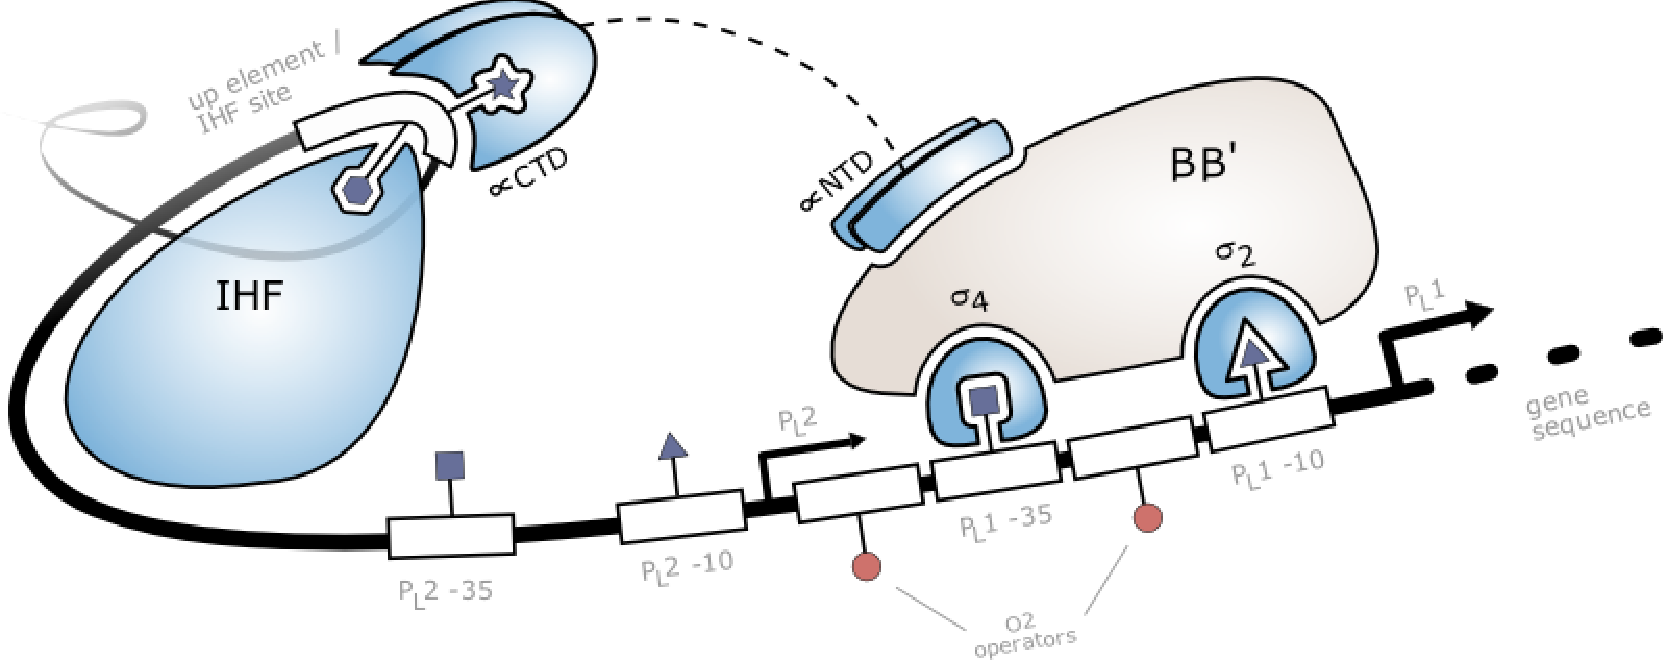
\includegraphics[width=\textwidth]{figures/fig1}
\caption[Short figure name.]{This is a figure that floats inline and here is its caption.
\label{fig:myInlineFigure}}
\end{figure}


Quisque facilisis erat a dui. Nam malesuada ornare dolor. Cras gravida, diam sit amet rhoncus ornare, erat elit consectetuer erat, id egestas pede nibh eget odio. Proin tincidunt, velit vel porta elementum, magna diam molestie sapien, non aliquet massa pede eu diam. Aliquam iaculis. Fusce et ipsum et nulla tristique facilisis. Donec eget sem sit amet ligula viverra gravida. Etiam vehicula urna vel turpis. Suspendisse sagittis ante a urna. Morbi a est quis orci consequat rutrum. Nullam egestas feugiat felis. Integer adipiscing semper ligula. Nunc molestie, nisl sit amet cursus convallis, sapien lectus pretium metus, vitae pretium enim wisi id lectus. Donec vestibulum. Etiam vel nibh. Nulla facilisi. Mauris pharetra. Donec augue. Fusce ultrices, neque id dignissim ultrices, tellus mauris dictum elit, vel lacinia enim metus eu nunc.

Proin at eros non eros adipiscing mollis. Donec semper turpis sed diam. Sed consequat ligula nec tortor. Integer eget sem. Ut vitae enim eu est vehicula gravida. Morbi ipsum ipsum, porta nec, tempor id, auctor vitae, purus. Pellentesque neque. Nulla luctus erat vitae libero. Integer nec enim. Phasellus aliquam enim et tortor. Quisque aliquet, quam elementum condimentum feugiat, tellus odio consectetuer wisi, vel nonummy sem neque in elit. Curabitur eleifend wisi iaculis ipsum. Pellentesque habitant morbi tristique senectus et netus et malesuada fames ac turpis egestas. In non velit non ligula laoreet ultrices. Praesent ultricies facilisis nisl. Vivamus luctus elit sit amet mi. Phasellus pellentesque, erat eget elementum volutpat, dolor nisl porta neque, vitae sodales ipsum nibh in ligula. Maecenas mattis pulvinar diam. Curabitur sed leo.

Nulla facilisi. In vel sem. Morbi id urna in diam dignissim feugiat. Proin molestie tortor eu velit. Aliquam erat volutpat. Nullam ultrices, diam tempus vulputate egestas, eros pede varius leo, sed imperdiet lectus est ornare odio. Lorem ipsum dolor sit amet, consectetuer adipiscing elit. Proin consectetuer velit in dui. Phasellus wisi purus, interdum vitae, rutrum accumsan, viverra in, velit. Sed enim risus, congue non, tristique in, commodo eu, metus. Aenean tortor mi, imperdiet id, gravida eu, posuere eu, felis. Mauris sollicitudin, turpis in hendrerit sodales, lectus ipsum pellentesque ligula, sit amet scelerisque urna nibh ut arcu. Aliquam in lacus. Vestibulum ante ipsum primis in faucibus orci luctus et ultrices posuere cubilia Curae; Nulla placerat aliquam wisi. Mauris viverra odio. Quisque fermentum pulvinar odio. Proin posuere est vitae ligula. Etiam euismod. Cras a eros.

Nunc auctor bibendum eros. Maecenas porta accumsan mauris. Etiam enim enim, elementum sed, bibendum quis, rhoncus non, metus. Fusce neque dolor, adipiscing sed, consectetuer et, lacinia sit amet, quam. Suspendisse wisi quam, consectetuer in, blandit sed, suscipit eu, eros. Etiam ligula enim, tempor ut, blandit nec, mollis eu, lectus. Nam cursus. Vivamus iaculis. Aenean risus purus, pharetra in, blandit quis, gravida a, turpis. Donec nisl. Aenean eget mi. Fusce mattis est id diam. Phasellus faucibus interdum sapien. Duis quis nunc. Sed enim.

Pellentesque vel dui sed orci faucibus iaculis. Suspendisse dictum magna id purus tincidunt rutrum. Nulla congue. Vivamus sit amet lorem posuere dui vulputate ornare. Phasellus mattis sollicitudin ligula. Duis dignissim felis et urna. Integer adipiscing congue metus. Nam pede. Etiam non wisi. Sed accumsan dolor ac augue. Pellentesque eget lectus. Aliquam nec dolor nec tellus ornare venenatis. Nullam blandit placerat sem. Curabitur quis ipsum. Mauris nisl tellus, aliquet eu, suscipit eu, ullamcorper quis, magna. Mauris elementum, pede at sodales vestibulum, nulla tortor congue massa, quis pellentesque odio dui id est. Cras faucibus augue.

%% Requires fltpage2 package
%%
% \begin{FPfigure}
% 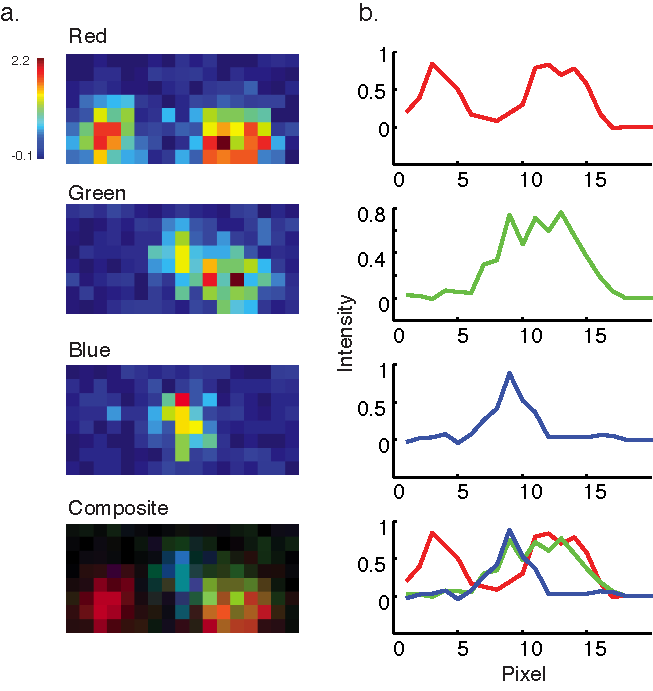
\includegraphics[width=\textwidth]{figures/fullpage}
% \caption[Short figure name.]{This is a full page figure using the FPfigure command. It takes up the whole page and the caption appears on the preceding page. Its useful for large figures. Harvard's rules about full page figures are tricky, but you don't have to worry about it because we took care of it for you. For example, the full figure is supposed to have a title in the same style as the caption but without the actual caption. The caption is supposed to appear alone on the preceding page with no other text. You do't have to worry about any of that. We have modified the fltpage package to make it work. This is a lengthy caption and it clearly would not fit on the same page as the figure. Note that you should only use the FPfigure command in instances where the figure really is too large. If the figure is small enough to fit by the caption than it does not produce the desired effect. Good luck with your thesis. I have to keep writing this to make the caption really long. LaTex is a lot of fun. You will enjoy working with it. Good luck on your post doctoral life! I am looking forward to mine. \label{fig:myFullPageFigure}}
% \end{FPfigure}
% \afterpage{\clearpage}

Suspendisse vestibulum dignissim quam. Integer vel augue. Phasellus nulla purus, interdum ac, venenatis non, varius rutrum, leo. Pellentesque habitant morbi tristique senectus et netus et malesuada fames ac turpis egestas. Duis a eros. Class aptent taciti sociosqu ad litora torquent per conubia nostra, per inceptos hymenaeos. Fusce magna mi, porttitor quis, convallis eget, sodales ac, urna. Phasellus luctus venenatis magna. Vivamus eget lacus. Nunc tincidunt convallis tortor. Duis eros mi, dictum vel, fringilla sit amet, fermentum id, sem. Phasellus nunc enim, faucibus ut, laoreet in, consequat id, metus. Vivamus dignissim. Cras lobortis tempor velit. Phasellus nec diam ac nisl lacinia tristique. Nullam nec metus id mi dictum dignissim. Nullam quis wisi non sem lobortis condimentum. Phasellus pulvinar, nulla non aliquam eleifend, tortor wisi scelerisque felis, in sollicitudin arcu ante lacinia leo.

Pellentesque habitant morbi tristique senectus et netus et malesuada fames ac turpis egestas. Vestibulum tortor quam, feugiat vitae, ultricies eget, tempor sit amet, ante. Donec eu libero sit amet quam egestas semper. Aenean ultricies mi vitae est. Mauris placerat eleifend leo. Quisque sit amet est et sapien ullamcorper pharetra. Vestibulum erat wisi, condimentum sed, commodo vitae, ornare sit amet, wisi. Aenean fermentum, elit eget tincidunt condimentum, eros ipsum rutrum orci, sagittis tempus lacus enim ac dui. Donec non enim in turpis pulvinar facilisis. Ut felis.

Cras sed ante. Phasellus in massa. Curabitur dolor eros, gravida et, hendrerit ac, cursus non, massa. Aliquam lorem. In hac habitasse platea dictumst. Cras eu mauris. Quisque lacus. Donec ipsum. Nullam vitae sem at nunc pharetra ultricies. Vivamus elit eros, ullamcorper a, adipiscing sit amet, porttitor ut, nibh. Maecenas adipiscing mollis massa. Nunc ut dui eget nulla venenatis aliquet. Sed luctus posuere justo. Cras vehicula varius turpis. Vivamus eros metus, tristique sit amet, molestie dignissim, malesuada et, urna.

Proin at eros non eros adipiscing mollis. Donec semper turpis sed diam. Sed consequat ligula nec tortor. Integer eget sem. Ut vitae enim eu est vehicula gravida. Morbi ipsum ipsum, porta nec, tempor id, auctor vitae, purus. Pellentesque neque. Nulla luctus erat vitae libero. Integer nec enim. Phasellus aliquam enim et tortor. Quisque aliquet, quam elementum condimentum feugiat, tellus odio consectetuer wisi, vel nonummy sem neque in elit. Curabitur eleifend wisi iaculis ipsum. Pellentesque habitant morbi tristique senectus et netus et malesuada fames ac turpis egestas. In non velit non ligula laoreet ultrices. Praesent ultricies facilisis nisl. Vivamus luctus elit sit amet mi. Phasellus pellentesque, erat eget elementum volutpat, dolor nisl porta neque, vitae sodales ipsum nibh in ligula. Maecenas mattis pulvinar diam. Curabitur sed leo.

Nulla facilisi. In vel sem. Morbi id urna in diam dignissim feugiat. Proin molestie tortor eu velit. Aliquam erat volutpat. Nullam ultrices, diam tempus vulputate egestas, eros pede varius leo, sed imperdiet lectus est ornare odio. Lorem ipsum dolor sit amet, consectetuer adipiscing elit. Proin consectetuer velit in dui. Phasellus wisi purus, interdum vitae, rutrum accumsan, viverra in, velit. Sed enim risus, congue non, tristique in, commodo eu, metus. Aenean tortor mi, imperdiet id, gravida eu, posuere eu, felis. Mauris sollicitudin, turpis in hendrerit sodales, lectus ipsum pellentesque ligula, sit amet scelerisque urna nibh ut arcu. Aliquam in lacus. Vestibulum ante ipsum primis in faucibus orci luctus et ultrices posuere cubilia Curae; Nulla placerat aliquam wisi. Mauris viverra odio. Quisque fermentum pulvinar odio. Proin posuere est vitae ligula. Etiam euismod. Cras a eros.

Nunc auctor bibendum eros. Maecenas porta accumsan mauris. Etiam enim enim, elementum sed, bibendum quis, rhoncus non, metus. Fusce neque dolor, adipiscing sed, consectetuer et, lacinia sit amet, quam. Suspendisse wisi quam, consectetuer in, blandit sed, suscipit eu, eros. Etiam ligula enim, tempor ut, blandit nec, mollis eu, lectus. Nam cursus. Vivamus iaculis. Aenean risus purus, pharetra in, blandit quis, gravida a, turpis. Donec nisl. Aenean eget mi. Fusce mattis est id diam. Phasellus faucibus interdum sapien. Duis quis nunc. Sed enim.

Pellentesque vel dui sed orci faucibus iaculis. Suspendisse dictum magna id purus tincidunt rutrum. Nulla congue. Vivamus sit amet lorem posuere dui vulputate ornare. Phasellus mattis sollicitudin ligula. Duis dignissim felis et urna. Integer adipiscing congue metus. Nam pede. Etiam non wisi. Sed accumsan dolor ac augue. Pellentesque eget lectus. Aliquam nec dolor nec tellus ornare venenatis. Nullam blandit placerat sem. Curabitur quis ipsum. Mauris nisl tellus, aliquet eu, suscipit eu, ullamcorper quis, magna. Mauris elementum, pede at sodales vestibulum, nulla tortor congue massa, quis pellentesque odio dui id est. Cras faucibus augue.

Suspendisse vestibulum dignissim quam. Integer vel augue. Phasellus nulla purus, interdum ac, venenatis non, varius rutrum, leo. Pellentesque habitant morbi tristique senectus et netus et malesuada fames ac turpis egestas. Duis a eros. Class aptent taciti sociosqu ad litora torquent per conubia nostra, per inceptos hymenaeos. Fusce magna mi, porttitor quis, convallis eget, sodales ac, urna. Phasellus luctus venenatis magna. Vivamus eget lacus. Nunc tincidunt convallis tortor. Duis eros mi, dictum vel, fringilla sit amet, fermentum id, sem. Phasellus nunc enim, faucibus ut, laoreet in, consequat id, metus. Vivamus dignissim. Cras lobortis tempor velit. Phasellus nec diam ac nisl lacinia tristique. Nullam nec metus id mi dictum dignissim. Nullam quis wisi non sem lobortis condimentum. Phasellus pulvinar, nulla non aliquam eleifend, tortor wisi scelerisque felis, in sollicitudin arcu ante lacinia leo.

Pellentesque habitant morbi tristique senectus et netus et malesuada fames ac turpis egestas. Vestibulum tortor quam, feugiat vitae, ultricies eget, tempor sit amet, ante. Donec eu libero sit amet quam egestas semper. Aenean ultricies mi vitae est. Mauris placerat eleifend leo. Quisque sit amet est et sapien ullamcorper pharetra. Vestibulum erat wisi, condimentum sed, commodo vitae, ornare sit amet, wisi. Aenean fermentum, elit eget tincidunt condimentum, eros ipsum rutrum orci, sagittis tempus lacus enim ac dui. Donec non enim in turpis pulvinar facilisis. Ut felis.

Cras sed ante. Phasellus in massa. Curabitur dolor eros, gravida et, hendrerit ac, cursus non, massa. Aliquam lorem. In hac habitasse platea dictumst. Cras eu mauris. Quisque lacus. Donec ipsum. Nullam vitae sem at nunc pharetra ultricies. Vivamus elit eros, ullamcorper a, adipiscing sit amet, porttitor ut, nibh. Maecenas adipiscing mollis massa. Nunc ut dui eget nulla venenatis aliquet. Sed luctus posuere justo. Cras vehicula varius turpis. Vivamus eros metus, tristique sit amet, molestie dignissim, malesuada et, urna.

Cras dictum. Maecenas ut turpis. In vitae erat ac orci dignissim eleifend. Nunc quis justo. Sed vel ipsum in purus tincidunt pharetra. Sed pulvinar, felis id consectetuer malesuada, enim nisl mattis elit, a facilisis tortor nibh quis leo. Sed augue lacus, pretium vitae, molestie eget, rhoncus quis, elit. Donec in augue. Fusce orci wisi, ornare id, mollis vel, lacinia vel, massa.

Lorem ipsum dolor sit amet, consectetuer adipiscing elit. Morbi commodo, ipsum sed pharetra gravida, orci magna rhoncus neque, id pulvinar odio lorem non turpis. Nullam sit amet enim. Suspendisse id velit vitae ligula volutpat condimentum. Aliquam erat volutpat. Sed quis velit. Nulla facilisi. Nulla libero. Vivamus pharetra posuere sapien. Nam consectetuer. Sed aliquam, nunc eget euismod ullamcorper, lectus nunc ullamcorper orci, fermentum bibendum enim nibh eget ipsum. Donec porttitor ligula eu dolor. Maecenas vitae nulla consequat libero cursus venenatis. Nam magna enim, accumsan eu, blandit sed, blandit a, eros.

Quisque facilisis erat a dui. Nam malesuada ornare dolor. Cras gravida, diam sit amet rhoncus ornare, erat elit consectetuer erat, id egestas pede nibh eget odio. Proin tincidunt, velit vel porta elementum, magna diam molestie sapien, non aliquet massa pede eu diam. Aliquam iaculis. Fusce et ipsum et nulla tristique facilisis. Donec eget sem sit amet ligula viverra gravida. Etiam vehicula urna vel turpis. Suspendisse sagittis ante a urna. Morbi a est quis orci consequat rutrum. Nullam egestas feugiat felis. Integer adipiscing semper ligula. Nunc molestie, nisl sit amet cursus convallis, sapien lectus pretium metus, vitae pretium enim wisi id lectus. Donec vestibulum. Etiam vel nibh. Nulla facilisi. Mauris pharetra. Donec augue. Fusce ultrices, neque id dignissim ultrices, tellus mauris dictum elit, vel lacinia enim metus eu nunc.

Proin at eros non eros adipiscing mollis. Donec semper turpis sed diam. Sed consequat ligula nec tortor. Integer eget sem. Ut vitae enim eu est vehicula gravida. Morbi ipsum ipsum, porta nec, tempor id, auctor vitae, purus. Pellentesque neque. Nulla luctus erat vitae libero. Integer nec enim. Phasellus aliquam enim et tortor. Quisque aliquet, quam elementum condimentum feugiat, tellus odio consectetuer wisi, vel nonummy sem neque in elit. Curabitur eleifend wisi iaculis ipsum. Pellentesque habitant morbi tristique senectus et netus et malesuada fames ac turpis egestas. In non velit non ligula laoreet ultrices. Praesent ultricies facilisis nisl. Vivamus luctus elit sit amet mi. Phasellus pellentesque, erat eget elementum volutpat, dolor nisl porta neque, vitae sodales ipsum nibh in ligula. Maecenas mattis pulvinar diam. Curabitur sed leo.

Nulla facilisi. In vel sem. Morbi id urna in diam dignissim feugiat. Proin molestie tortor eu velit. Aliquam erat volutpat. Nullam ultrices, diam tempus vulputate egestas, eros pede varius leo, sed imperdiet lectus est ornare odio. Lorem ipsum dolor sit amet, consectetuer adipiscing elit. Proin consectetuer velit in dui. Phasellus wisi purus, interdum vitae, rutrum accumsan, viverra in, velit. Sed enim risus, congue non, tristique in, commodo eu, metus. Aenean tortor mi, imperdiet id, gravida eu, posuere eu, felis. Mauris sollicitudin, turpis in hendrerit sodales, lectus ipsum pellentesque ligula, sit amet scelerisque urna nibh ut arcu. Aliquam in lacus. Vestibulum ante ipsum primis in faucibus orci luctus et ultrices posuere cubilia Curae; Nulla placerat aliquam wisi. Mauris viverra odio. Quisque fermentum pulvinar odio. Proin posuere est vitae ligula. Etiam euismod. Cras a eros.

Nunc auctor bibendum eros. Maecenas porta accumsan mauris. Etiam enim enim, elementum sed, bibendum quis, rhoncus non, metus. Fusce neque dolor, adipiscing sed, consectetuer et, lacinia sit amet, quam. Suspendisse wisi quam, consectetuer in, blandit sed, suscipit eu, eros. Etiam ligula enim, tempor ut, blandit nec, mollis eu, lectus. Nam cursus. Vivamus iaculis. Aenean risus purus, pharetra in, blandit quis, gravida a, turpis. Donec nisl. Aenean eget mi. Fusce mattis est id diam. Phasellus faucibus interdum sapien. Duis quis nunc. Sed enim.

Pellentesque vel dui sed orci faucibus iaculis. Suspendisse dictum magna id purus tincidunt rutrum. Nulla congue. Vivamus sit amet lorem posuere dui vulputate ornare. Phasellus mattis sollicitudin ligula. Duis dignissim felis et urna. Integer adipiscing congue metus. Nam pede. Etiam non wisi. Sed accumsan dolor ac augue. Pellentesque eget lectus. Aliquam nec dolor nec tellus ornare venenatis. Nullam blandit placerat sem. Curabitur quis ipsum. Mauris nisl tellus, aliquet eu, suscipit eu, ullamcorper quis, magna. Mauris elementum, pede at sodales vestibulum, nulla tortor congue massa, quis pellentesque odio dui id est. Cras faucibus augue.

Suspendisse vestibulum dignissim quam. Integer vel augue. Phasellus nulla purus, interdum ac, venenatis non, varius rutrum, leo. Pellentesque habitant morbi tristique senectus et netus et malesuada fames ac turpis egestas. Duis a eros. Class aptent taciti sociosqu ad litora torquent per conubia nostra, per inceptos hymenaeos. Fusce magna mi, porttitor quis, convallis eget, sodales ac, urna. Phasellus luctus venenatis magna. Vivamus eget lacus. Nunc tincidunt convallis tortor. Duis eros mi, dictum vel, fringilla sit amet, fermentum id, sem. Phasellus nunc enim, faucibus ut, laoreet in, consequat id, metus. Vivamus dignissim. Cras lobortis tempor velit. Phasellus nec diam ac nisl lacinia tristique. Nullam nec metus id mi dictum dignissim. Nullam quis wisi non sem lobortis condimentum. Phasellus pulvinar, nulla non aliquam eleifend, tortor wisi scelerisque felis, in sollicitudin arcu ante lacinia leo.

Pellentesque habitant morbi tristique senectus et netus et malesuada fames ac turpis egestas. Vestibulum tortor quam, feugiat vitae, ultricies eget, tempor sit amet, ante. Donec eu libero sit amet quam egestas semper. Aenean ultricies mi vitae est. Mauris placerat eleifend leo. Quisque sit amet est et sapien ullamcorper pharetra. Vestibulum erat wisi, condimentum sed, commodo vitae, ornare sit amet, wisi. Aenean fermentum, elit eget tincidunt condimentum, eros ipsum rutrum orci, sagittis tempus lacus enim ac dui. Donec non enim in turpis pulvinar facilisis. Ut felis.

Cras sed ante. Phasellus in massa. Curabitur dolor eros, gravida et, hendrerit ac, cursus non, massa. Aliquam lorem. In hac habitasse platea dictumst. Cras eu mauris. Quisque lacus. Donec ipsum. Nullam vitae sem at nunc pharetra ultricies. Vivamus elit eros, ullamcorper a, adipiscing sit amet, porttitor ut, nibh. Maecenas adipiscing mollis massa. Nunc ut dui eget nulla venenatis aliquet. Sed luctus posuere justo. Cras vehicula varius turpis. Vivamus eros metus, tristique sit amet, molestie dignissim, malesuada et, urna.

Cras dictum. Maecenas ut turpis. In vitae erat ac orci dignissim eleifend. Nunc quis justo. Sed vel ipsum in purus tincidunt pharetra. Sed pulvinar, felis id consectetuer malesuada, enim nisl mattis elit, a facilisis tortor nibh quis leo. Sed augue lacus, pretium vitae, molestie eget, rhoncus quis, elit. Donec in augue. Fusce orci wisi, ornare id, mollis vel, lacinia vel, massa.

Lorem ipsum dolor sit amet, consectetuer adipiscing elit. Morbi commodo, ipsum sed pharetra gravida, orci magna rhoncus neque, id pulvinar odio lorem non turpis. Nullam sit amet enim. Suspendisse id velit vitae ligula volutpat condimentum. Aliquam erat volutpat. Sed quis velit. Nulla facilisi. Nulla libero. Vivamus pharetra posuere sapien. Nam consectetuer. Sed aliquam, nunc eget euismod ullamcorper, lectus nunc ullamcorper orci, fermentum bibendum enim nibh eget ipsum. Donec porttitor ligula eu dolor. Maecenas vitae nulla consequat libero cursus venenatis. Nam magna enim, accumsan eu, blandit sed, blandit a, eros.

Quisque facilisis erat a dui. Nam malesuada ornare dolor. Cras gravida, diam sit amet rhoncus ornare, erat elit consectetuer erat, id egestas pede nibh eget odio. Proin tincidunt, velit vel porta elementum, magna diam molestie sapien, non aliquet massa pede eu diam. Aliquam iaculis. Fusce et ipsum et nulla tristique facilisis. Donec eget sem sit amet ligula viverra gravida. Etiam vehicula urna vel turpis. Suspendisse sagittis ante a urna. Morbi a est quis orci consequat rutrum. Nullam egestas feugiat felis. Integer adipiscing semper ligula. Nunc molestie, nisl sit amet cursus convallis, sapien lectus pretium metus, vitae pretium enim wisi id lectus. Donec vestibulum. Etiam vel nibh. Nulla facilisi. Mauris pharetra. Donec augue. Fusce ultrices, neque id dignissim ultrices, tellus mauris dictum elit, vel lacinia enim metus eu nunc.

Proin at eros non eros adipiscing mollis. Donec semper turpis sed diam. Sed consequat ligula nec tortor. Integer eget sem. Ut vitae enim eu est vehicula gravida. Morbi ipsum ipsum, porta nec, tempor id, auctor vitae, purus. Pellentesque neque. Nulla luctus erat vitae libero. Integer nec enim. Phasellus aliquam enim et tortor. Quisque aliquet, quam elementum condimentum feugiat, tellus odio consectetuer wisi, vel nonummy sem neque in elit. Curabitur eleifend wisi iaculis ipsum. Pellentesque habitant morbi tristique senectus et netus et malesuada fames ac turpis egestas. In non velit non ligula laoreet ultrices. Praesent ultricies facilisis nisl. Vivamus luctus elit sit amet mi. Phasellus pellentesque, erat eget elementum volutpat, dolor nisl porta neque, vitae sodales ipsum nibh in ligula. Maecenas mattis pulvinar diam. Curabitur sed leo.

Nulla facilisi. In vel sem. Morbi id urna in diam dignissim feugiat. Proin molestie tortor eu velit. Aliquam erat volutpat. Nullam ultrices, diam tempus vulputate egestas, eros pede varius leo, sed imperdiet lectus est ornare odio. Lorem ipsum dolor sit amet, consectetuer adipiscing elit. Proin consectetuer velit in dui. Phasellus wisi purus, interdum vitae, rutrum accumsan, viverra in, velit. Sed enim risus, congue non, tristique in, commodo eu, metus. Aenean tortor mi, imperdiet id, gravida eu, posuere eu, felis. Mauris sollicitudin, turpis in hendrerit sodales, lectus ipsum pellentesque ligula, sit amet scelerisque urna nibh ut arcu. Aliquam in lacus. Vestibulum ante ipsum primis in faucibus orci luctus et ultrices posuere cubilia Curae; Nulla placerat aliquam wisi. Mauris viverra odio. Quisque fermentum pulvinar odio. Proin posuere est vitae ligula. Etiam euismod. Cras a eros.

Nunc auctor bibendum eros. Maecenas porta accumsan mauris. Etiam enim enim, elementum sed, bibendum quis, rhoncus non, metus. Fusce neque dolor, adipiscing sed, consectetuer et, lacinia sit amet, quam. Suspendisse wisi quam, consectetuer in, blandit sed, suscipit eu, eros. Etiam ligula enim, tempor ut, blandit nec, mollis eu, lectus. Nam cursus. Vivamus iaculis. Aenean risus purus, pharetra in, blandit quis, gravida a, turpis. Donec nisl. Aenean eget mi. Fusce mattis est id diam. Phasellus faucibus interdum sapien. Duis quis nunc. Sed enim.


Cras sed ante. Phasellus in massa. Curabitur dolor eros, gravida et, hendrerit ac, cursus non, massa. Aliquam lorem. In hac habitasse platea dictumst. Cras eu mauris. Quisque lacus. Donec ipsum. Nullam vitae sem at nunc pharetra ultricies. Vivamus elit eros, ullamcorper a, adipiscing sit amet, porttitor ut, nibh. Maecenas adipiscing mollis massa. Nunc ut dui eget nulla venenatis aliquet. Sed luctus posuere justo. Cras vehicula varius turpis. Vivamus eros metus, tristique sit amet, molestie dignissim, malesuada et, urna.

Cras dictum. Maecenas ut turpis. In vitae erat ac orci dignissim eleifend. Nunc quis justo. Sed vel ipsum in purus tincidunt pharetra. Sed pulvinar, felis id consectetuer malesuada, enim nisl mattis elit, a facilisis tortor nibh quis leo. Sed augue lacus, pretium vitae, molestie eget, rhoncus quis, elit. Donec in augue. Fusce orci wisi, ornare id, mollis vel, lacinia vel, massa.

Lorem ipsum dolor sit amet, consectetuer adipiscing elit. Morbi commodo, ipsum sed pharetra gravida, orci magna rhoncus neque, id pulvinar odio lorem non turpis. Nullam sit amet enim. Suspendisse id velit vitae ligula volutpat condimentum. Aliquam erat volutpat. Sed quis velit. Nulla facilisi. Nulla libero. Vivamus pharetra posuere sapien. Nam consectetuer. Sed aliquam, nunc eget euismod ullamcorper, lectus nunc ullamcorper orci, fermentum bibendum enim nibh eget ipsum. Donec porttitor ligula eu dolor. Maecenas vitae nulla consequat libero cursus venenatis. Nam magna enim, accumsan eu, blandit sed, blandit a, eros.

Quisque facilisis erat a dui. Nam malesuada ornare dolor. Cras gravida, diam sit amet rhoncus ornare, erat elit consectetuer erat, id egestas pede nibh eget odio. Proin tincidunt, velit vel porta elementum, magna diam molestie sapien, non aliquet massa pede eu diam. Aliquam iaculis. Fusce et ipsum et nulla tristique facilisis. Donec eget sem sit amet ligula viverra gravida. Etiam vehicula urna vel turpis. Suspendisse sagittis ante a urna. Morbi a est quis orci consequat rutrum. Nullam egestas feugiat felis. Integer adipiscing semper ligula. Nunc molestie, nisl sit amet cursus convallis, sapien lectus pretium metus, vitae pretium enim wisi id lectus. Donec vestibulum. Etiam vel nibh. Nulla facilisi. Mauris pharetra. Donec augue. Fusce ultrices, neque id dignissim ultrices, tellus mauris dictum elit, vel lacinia enim metus eu nunc.

Proin at eros non eros adipiscing mollis. Donec semper turpis sed diam. Sed consequat ligula nec tortor. Integer eget sem. Ut vitae enim eu est vehicula gravida. Morbi ipsum ipsum, porta nec, tempor id, auctor vitae, purus. Pellentesque neque. Nulla luctus erat vitae libero. Integer nec enim. Phasellus aliquam enim et tortor. Quisque aliquet, quam elementum condimentum feugiat, tellus odio consectetuer wisi, vel nonummy sem neque in elit. Curabitur eleifend wisi iaculis ipsum. Pellentesque habitant morbi tristique senectus et netus et malesuada fames ac turpis egestas. In non velit non ligula laoreet ultrices. Praesent ultricies facilisis nisl. Vivamus luctus elit sit amet mi. Phasellus pellentesque, erat eget elementum volutpat, dolor nisl porta neque, vitae sodales ipsum nibh in ligula. Maecenas mattis pulvinar diam. Curabitur sed leo.

Nulla facilisi. In vel sem. Morbi id urna in diam dignissim feugiat. Proin molestie tortor eu velit. Aliquam erat volutpat. Nullam ultrices, diam tempus vulputate egestas, eros pede varius leo, sed imperdiet lectus est ornare odio. Lorem ipsum dolor sit amet, consectetuer adipiscing elit. Proin consectetuer velit in dui. Phasellus wisi purus, interdum vitae, rutrum accumsan, viverra in, velit. Sed enim risus, congue non, tristique in, commodo eu, metus. Aenean tortor mi, imperdiet id, gravida eu, posuere eu, felis. Mauris sollicitudin, turpis in hendrerit sodales, lectus ipsum pellentesque ligula, sit amet scelerisque urna nibh ut arcu. Aliquam in lacus. Vestibulum ante ipsum primis in faucibus orci luctus et ultrices posuere cubilia Curae; Nulla placerat aliquam wisi. Mauris viverra odio. Quisque fermentum pulvinar odio. Proin posuere est vitae ligula. Etiam euismod. Cras a eros.

Nunc auctor bibendum eros. Maecenas porta accumsan mauris. Etiam enim enim, elementum sed, bibendum quis, rhoncus non, metus. Fusce neque dolor, adipiscing sed, consectetuer et, lacinia sit amet, quam. Suspendisse wisi quam, consectetuer in, blandit sed, suscipit eu, eros. Etiam ligula enim, tempor ut, blandit nec, mollis eu, lectus. Nam cursus. Vivamus iaculis. Aenean risus purus, pharetra in, blandit quis, gravida a, turpis. Donec nisl. Aenean eget mi. Fusce mattis est id diam. Phasellus faucibus interdum sapien. Duis quis nunc. Sed enim.

Pellentesque vel dui sed orci faucibus iaculis. Suspendisse dictum magna id purus tincidunt rutrum. Nulla congue. Vivamus sit amet lorem posuere dui vulputate ornare. Phasellus mattis sollicitudin ligula. Duis dignissim felis et urna. Integer adipiscing congue metus. Nam pede. Etiam non wisi. Sed accumsan dolor ac augue. Pellentesque eget lectus. Aliquam nec dolor nec tellus ornare venenatis. Nullam blandit placerat sem. Curabitur quis ipsum. Mauris nisl tellus, aliquet eu, suscipit eu, ullamcorper quis, magna. Mauris elementum, pede at sodales vestibulum, nulla tortor congue massa, quis pellentesque odio dui id est. Cras faucibus augue.

Suspendisse vestibulum dignissim quam. Integer vel augue. Phasellus nulla purus, interdum ac, venenatis non, varius rutrum, leo. Pellentesque habitant morbi tristique senectus et netus et malesuada fames ac turpis egestas. Duis a eros. Class aptent taciti sociosqu ad litora torquent per conubia nostra, per inceptos hymenaeos. Fusce magna mi, porttitor quis, convallis eget, sodales ac, urna. Phasellus luctus venenatis magna. Vivamus eget lacus. Nunc tincidunt convallis tortor. Duis eros mi, dictum vel, fringilla sit amet, fermentum id, sem. Phasellus nunc enim, faucibus ut, laoreet in, consequat id, metus. Vivamus dignissim. Cras lobortis tempor velit. Phasellus nec diam ac nisl lacinia tristique. Nullam nec metus id mi dictum dignissim. Nullam quis wisi non sem lobortis condimentum. Phasellus pulvinar, nulla non aliquam eleifend, tortor wisi scelerisque felis, in sollicitudin arcu ante lacinia leo.

Pellentesque habitant morbi tristique senectus et netus et malesuada fames ac turpis egestas. Vestibulum tortor quam, feugiat vitae, ultricies eget, tempor sit amet, ante. Donec eu libero sit amet quam egestas semper. Aenean ultricies mi vitae est. Mauris placerat eleifend leo. Quisque sit amet est et sapien ullamcorper pharetra. Vestibulum erat wisi, condimentum sed, commodo vitae, ornare sit amet, wisi. Aenean fermentum, elit eget tincidunt condimentum, eros ipsum rutrum orci, sagittis tempus lacus enim ac dui. Donec non enim in turpis pulvinar facilisis. Ut felis.

Cras sed ante. Phasellus in massa. Curabitur dolor eros, gravida et, hendrerit ac, cursus non, massa. Aliquam lorem. In hac habitasse platea dictumst. Cras eu mauris. Quisque lacus. Donec ipsum. Nullam vitae sem at nunc pharetra ultricies. Vivamus elit eros, ullamcorper a, adipiscing sit amet, porttitor ut, nibh. Maecenas adipiscing mollis massa. Nunc ut dui eget nulla venenatis aliquet. Sed luctus posuere justo. Cras vehicula varius turpis. Vivamus eros metus, tristique sit amet, molestie dignissim, malesuada et, urna.

Cras dictum. Maecenas ut turpis. In vitae erat ac orci dignissim eleifend. Nunc quis justo. Sed vel ipsum in purus tincidunt pharetra. Sed pulvinar, felis id consectetuer malesuada, enim nisl mattis elit, a facilisis tortor nibh quis leo. Sed augue lacus, pretium vitae, molestie eget, rhoncus quis, elit. Donec in augue. Fusce orci wisi, ornare id, mollis vel, lacinia vel, massa.

Lorem ipsum dolor sit amet, consectetuer adipiscing elit. Morbi commodo, ipsum sed pharetra gravida, orci magna rhoncus neque, id pulvinar odio lorem non turpis. Nullam sit amet enim. Suspendisse id velit vitae ligula volutpat condimentum. Aliquam erat volutpat. Sed quis velit. Nulla facilisi. Nulla libero. Vivamus pharetra posuere sapien. Nam consectetuer. Sed aliquam, nunc eget euismod ullamcorper, lectus nunc ullamcorper orci, fermentum bibendum enim nibh eget ipsum. Donec porttitor ligula eu dolor. Maecenas vitae nulla consequat libero cursus venenatis. Nam magna enim, accumsan eu, blandit sed, blandit a, eros.

Quisque facilisis erat a dui. Nam malesuada ornare dolor. Cras gravida, diam sit amet rhoncus ornare, erat elit consectetuer erat, id egestas pede nibh eget odio. Proin tincidunt, velit vel porta elementum, magna diam molestie sapien, non aliquet massa pede eu diam. Aliquam iaculis. Fusce et ipsum et nulla tristique facilisis. Donec eget sem sit amet ligula viverra gravida. Etiam vehicula urna vel turpis. Suspendisse sagittis ante a urna. Morbi a est quis orci consequat rutrum. Nullam egestas feugiat felis. Integer adipiscing semper ligula. Nunc molestie, nisl sit amet cursus convallis, sapien lectus pretium metus, vitae pretium enim wisi id lectus. Donec vestibulum. Etiam vel nibh. Nulla facilisi. Mauris pharetra. Donec augue. Fusce ultrices, neque id dignissim ultrices, tellus mauris dictum elit, vel lacinia enim metus eu nunc.

Proin at eros non eros adipiscing mollis. Donec semper turpis sed diam. Sed consequat ligula nec tortor. Integer eget sem. Ut vitae enim eu est vehicula gravida. Morbi ipsum ipsum, porta nec, tempor id, auctor vitae, purus. Pellentesque neque. Nulla luctus erat vitae libero. Integer nec enim. Phasellus aliquam enim et tortor. Quisque aliquet, quam elementum condimentum feugiat, tellus odio consectetuer wisi, vel nonummy sem neque in elit. Curabitur eleifend wisi iaculis ipsum. Pellentesque habitant morbi tristique senectus et netus et malesuada fames ac turpis egestas. In non velit non ligula laoreet ultrices. Praesent ultricies facilisis nisl. Vivamus luctus elit sit amet mi. Phasellus pellentesque, erat eget elementum volutpat, dolor nisl porta neque, vitae sodales ipsum nibh in ligula. Maecenas mattis pulvinar diam. Curabitur sed leo.

Nulla facilisi. In vel sem. Morbi id urna in diam dignissim feugiat. Proin molestie tortor eu velit. Aliquam erat volutpat. Nullam ultrices, diam tempus vulputate egestas, eros pede varius leo, sed imperdiet lectus est ornare odio. Lorem ipsum dolor sit amet, consectetuer adipiscing elit. Proin consectetuer velit in dui. Phasellus wisi purus, interdum vitae, rutrum accumsan, viverra in, velit. Sed enim risus, congue non, tristique in, commodo eu, metus. Aenean tortor mi, imperdiet id, gravida eu, posuere eu, felis. Mauris sollicitudin, turpis in hendrerit sodales, lectus ipsum pellentesque ligula, sit amet scelerisque urna nibh ut arcu. Aliquam in lacus. Vestibulum ante ipsum primis in faucibus orci luctus et ultrices posuere cubilia Curae; Nulla placerat aliquam wisi. Mauris viverra odio. Quisque fermentum pulvinar odio. Proin posuere est vitae ligula. Etiam euismod. Cras a eros.

Nunc auctor bibendum eros. Maecenas porta accumsan mauris. Etiam enim enim, elementum sed, bibendum quis, rhoncus non, metus. Fusce neque dolor, adipiscing sed, consectetuer et, lacinia sit amet, quam. Suspendisse wisi quam, consectetuer in, blandit sed, suscipit eu, eros. Etiam ligula enim, tempor ut, blandit nec, mollis eu, lectus. Nam cursus. Vivamus iaculis. Aenean risus purus, pharetra in, blandit quis, gravida a, turpis. Donec nisl. Aenean eget mi. Fusce mattis est id diam. Phasellus faucibus interdum sapien. Duis quis nunc. Sed enim.

Pellentesque vel dui sed orci faucibus iaculis. Suspendisse dictum magna id purus tincidunt rutrum. Nulla congue. Vivamus sit amet lorem posuere dui vulputate ornare. Phasellus mattis sollicitudin ligula. Duis dignissim felis et urna. Integer adipiscing congue metus. Nam pede. Etiam non wisi. Sed accumsan dolor ac augue. Pellentesque eget lectus. Aliquam nec dolor nec tellus ornare venenatis. Nullam blandit placerat sem. Curabitur quis ipsum. Mauris nisl tellus, aliquet eu, suscipit eu, ullamcorper quis, magna. Mauris elementum, pede at sodales vestibulum, nulla tortor congue massa, quis pellentesque odio dui id est. Cras faucibus augue.

Suspendisse vestibulum dignissim quam. Integer vel augue. Phasellus nulla purus, interdum ac, venenatis non, varius rutrum, leo. Pellentesque habitant morbi tristique senectus et netus et malesuada fames ac turpis egestas. Duis a eros. Class aptent taciti sociosqu ad litora torquent per conubia nostra, per inceptos hymenaeos. Fusce magna mi, porttitor quis, convallis eget, sodales ac, urna. Phasellus luctus venenatis magna. Vivamus eget lacus. Nunc tincidunt convallis tortor. Duis eros mi, dictum vel, fringilla sit amet, fermentum id, sem. Phasellus nunc enim, faucibus ut, laoreet in, consequat id, metus. Vivamus dignissim. Cras lobortis tempor velit. Phasellus nec diam ac nisl lacinia tristique. Nullam nec metus id mi dictum dignissim. Nullam quis wisi non sem lobortis condimentum. Phasellus pulvinar, nulla non aliquam eleifend, tortor wisi scelerisque felis, in sollicitudin arcu ante lacinia leo.
         % for clarity, we split the source into several files
%# -*- coding: utf-8-unix -*-
%%==================================================

\chapter{{\LaTeX} 排版例子}

\section{数学排版}

\subsection{公式排版}

这里有举一个长公式排版的例子,来自\href{http://www.tex.ac.uk/tex-archive/info/math/voss/mathmode/Mathmode.pdf}{《Math mode》}:

\begin{multline}
  \frac {1}{2}\Delta (f_{ij}f^{ij})=
  2\left (\sum _{i<j}\chi _{ij}(\sigma _{i}-
    \sigma _{j}) ^{2}+ f^{ij}\nabla _{j}\nabla _{i}(\Delta f)+\right .\\
  \left .+\nabla _{k}f_{ij}\nabla ^{k}f^{ij}+
    f^{ij}f^{k}\left [2\nabla _{i}R_{jk}-
      \nabla _{k}R_{ij}\right ]\vphantom {\sum _{i<j}}\right )
\end{multline}

下面演示了mathtools宏包中可伸长符号(箭头、等号的例子)的例子。
\begin{displaymath}
A \xleftarrow[n=0]{} B \xrightarrow[LongLongLongLong]{n>0} C 
\end{displaymath}

\begin{eqnarray}
f(x) & \xleftrightarrow[]{A=B}  & B \\
& \xleftharpoondown[below]{above} & B \nonumber \\
& \xLeftrightarrow[below]{above} & B
\end{eqnarray}

又如:
\begin{align}
\label{eq:none}
& I(X_3;X_4)-I(X_3;X_4\mid{}X_1)-I(X_3;X_4\mid{}X_2) \nonumber \\
= & [I(X_3;X_4)-I(X_3;X_4\mid{}X_1)]-I(X_3;X_4\mid{}\tilde{X}_2) \\
= & I(X_1;X_3;X_4)-I(X_3;X_4\mid{}\tilde{X}_2)
\end{align}

\subsection{国际单位制}

使用\verb+siunitx+宏包可以方便地输入国际标准单位制单位,例如\verb+\SI{5}{\um}+可以得到\SI{5}{\um}。

\subsection{定理环境}

模板中定义了丰富的定理环境
algo(算法),thm(定理),lem(引理),prop(命题),cor(推论),defn(定义),conj(猜想),exmp(例),rem(注),case(情形),
bthm(断言定理),blem(断言引理),bprop(断言命题),bcor(断言推论)。
amsmath还提供了一个proof(证明)的环境。
这里举一个“定理”和“证明”的例子。
\begin{thm}[留数定理]
\label{thm:res}
  假设$U$是复平面上的一个单连通开子集,$a_1,\ldots,a_n$是复平面上有限个点,$f$是定义在$U\backslash \{a_1,\ldots,a_n\}$上的全纯函数,
  如果$\gamma$是一条把$a_1,\ldots,a_n$包围起来的可求长曲线,但不经过任何一个$a_k$,并且其起点与终点重合,那么:

  \begin{equation}
    \label{eq:res}
    \ointop_{\gamma}f(z)\,\mathrm{d}z = 2\uppi\mathbf{i}\sum^n_{k=1}\mathrm{I}(\gamma,a_k)\mathrm{Res}(f,a_k)
  \end{equation}

  如果$\gamma$是若尔当曲线,那么$\mathrm{I}(\gamma, a_k)=1$,因此:

  \begin{equation}
    \label{eq:resthm}
    \ointop_{\gamma}f(z)\,\mathrm{d}z = 2\uppi\mathbf{i}\sum^n_{k=1}\mathrm{Res}(f,a_k)
  \end{equation}

      % \oint_\gamma f(z)\, dz = 2\pi i \sum_{k=1}^n \mathrm{Res}(f, a_k ). 

  在这里,$\mathrm{Res}(f, a_k)$表示$f$在点$a_k$的留数,$\mathrm{I}(\gamma,a_k)$表示$\gamma$关于点$a_k$的卷绕数。
  卷绕数是一个整数,它描述了曲线$\gamma$绕过点$a_k$的次数。如果$\gamma$依逆时针方向绕着$a_k$移动,卷绕数就是一个正数,
  如果$\gamma$根本不绕过$a_k$,卷绕数就是零。

  定理\ref{thm:res}的证明。
  
  \begin{proof}
    首先,由……

    其次,……

    所以……
  \end{proof}
\end{thm}

上面的公式例子中,有一些细节希望大家注意。微分号d应该使用“直立体”也就是用mathrm包围起来。
并且,微分号和被积函数之间应该有一段小间隔,可以插入\verb+\,+得到。
斜体的$d$通常只作为一般变量。
i,j作为虚数单位时,也应该使用“直立体”为了明显,还加上了粗体,例如\verb+\mathbf{i}+。斜体$i,j$通常用作表示“序号”。
其他字母在表示常量时,也推荐使用“直立体”譬如,圆周率$\uppi$(需要upgreek宏包),自然对数的底$\mathrm{e}$。
不过,我个人觉得斜体的$e$和$\pi$很潇洒,在不至于引起混淆的情况下,我也用这两个字母的斜体表示对应的常量。

\section{插入图像}

\subsection{支持的图片格式}

\XeTeX 可以很方便地插入PDF、PNG、JPG格式的图片。

JPG的例子如\ref{fig:csulogo}所示,PNG的例子如\ref{fig:tem}所示,
\begin{figure}[!htp]
  \centering
  
\includegraphics[scale=0.4]{example/csulogo.jpg}
  \caption{中南大学校徽}
  \label{fig:csulogo}
\end{figure}

\begin{figure}[!htp]
	\centering
	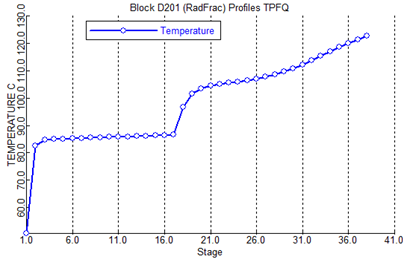
\includegraphics[scale=0.6]{example/tem.png}
	\caption{塔板温度分布图}
	\label{fig:tem}
\end{figure}

这里还有插入EPS图像和PDF图像的例子,如图\ref{fig:epspdf:a}和图\ref{fig:epspdf:b}。这里将EPS和PDF图片作为子图插入,每个子图有自己的小标题。子图标题使用subcaption宏包添加。

\begin{figure}[!htp]
  \centering
  \subcaptionbox{EPS 图像\label{fig:epspdf:a}}[3cm] %标题的长度,超过则会换行,如下一个小图。
    {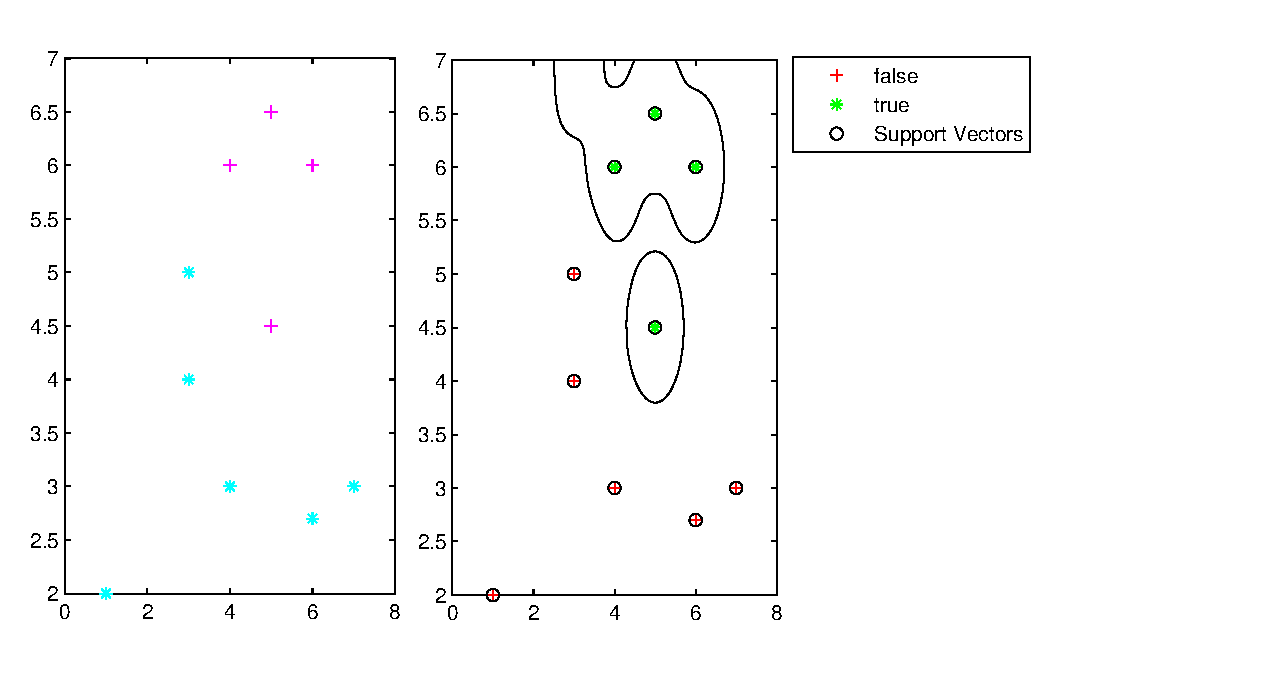
\includegraphics[height=4cm]{example/fig14.eps}}
  \hspace{4em}
  \subcaptionbox{PDF 图像。如果标题很长的话,它会自动换行\label{fig:epspdf:b}}
    {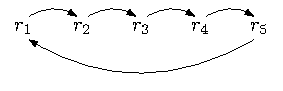
\includegraphics{example/permutation.pdf}}
  \caption{插入eps和pdf的例子(使用 subcaptionbox 方式)}
  \label{fig:pdfeps-subcaptionbox}
\end{figure}

\begin{figure}[!htp]
  \centering
  \begin{subfigure}{2.5cm}
    \centering
    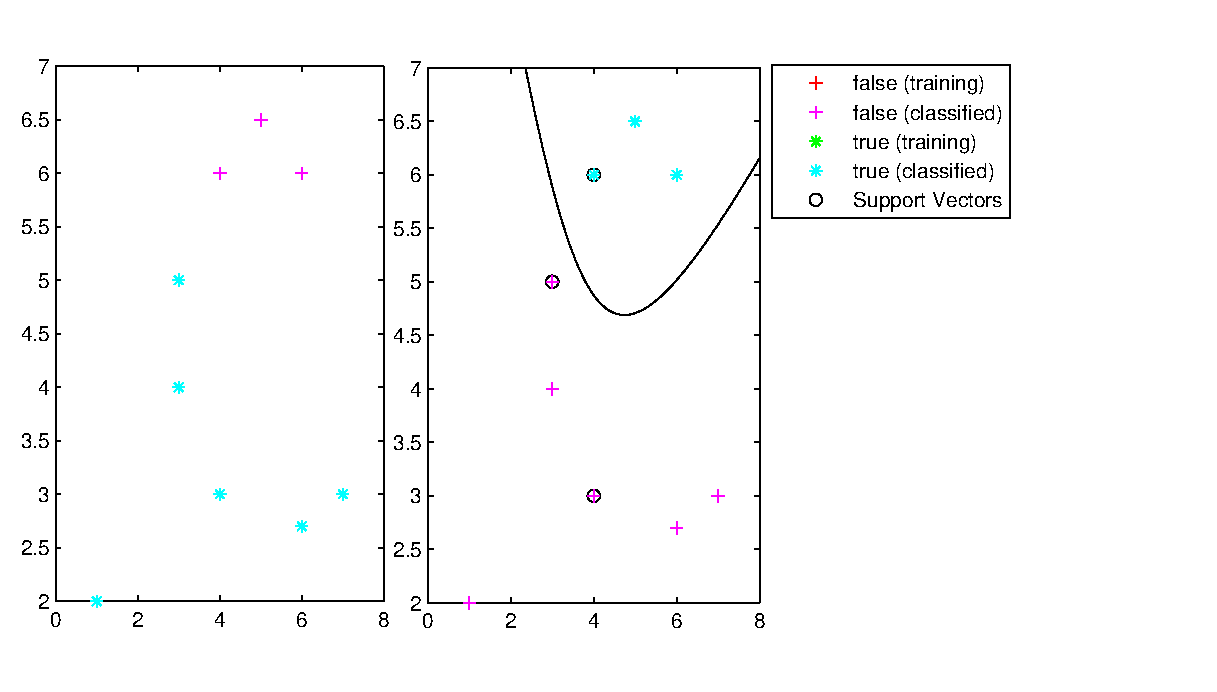
\includegraphics[height=3cm]{example/fig13.eps}
    \caption{EPS 图像}
  \end{subfigure}
  \hspace{4em}
  \begin{subfigure}{0.4\textwidth}
    \centering
    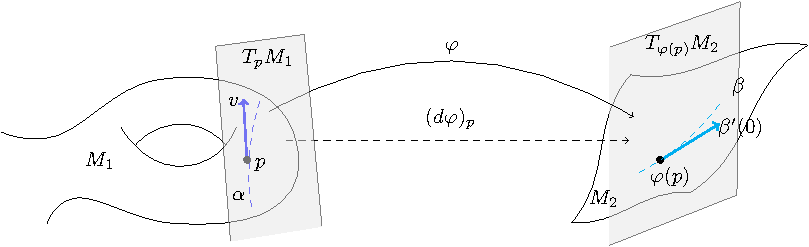
\includegraphics[height=2cm]{example/tangentmap.pdf}
    \caption{PDF 图像,注意这个图略矮些。subfigure中同一行的子图在顶端对齐。}
  \end{subfigure}
  \caption{插入eps和pdf的例子(使用 subfigure 方式)}
  \label{fig:pdfeps-subfigure}
\end{figure}

更多关于 \LaTeX 插图的例子可以参考\href{http://www.cs.duke.edu/junhu/Graphics3.pdf}{《\LaTeX 插图指南》}。

\subsection{绘制流程图}

图\ref{fig:flow_chart}是一张流程图示意。使用tikz环境,搭配四种预定义节点(\verb+startstop+、\verb+process+、\verb+decision+和\verb+io+),可以容易地绘制出流程图。
\begin{figure}[!htp]
    \centering
    \resizebox{6cm}{!}{\begin{tikzpicture}[node distance=2cm]
    \node (pic) [startstop] {待测图片};
    \node (bg) [io, below of=pic] {读取背景};
    \node (pair) [process, below of=bg] {匹配特征点对};
    \node (threshold) [decision, below of=pair, yshift=-0.5cm] {多于阈值};
    \node (clear) [decision, right of=threshold, xshift=3cm] {清晰?};
    \node (capture) [process, right of=pair, xshift=3cm, yshift=0.5cm] {重采};
    \node (matrix_p) [process, below of=threshold, yshift=-0.8cm] {透视变换矩阵};
    \node (matrix_a) [process, right of=matrix_p, xshift=3cm] {仿射变换矩阵};
    \node (reg) [process, below of=matrix_p] {图像修正};
    \node (return) [startstop, below of=reg] {配准结果};
     
    %连接具体形状
    \draw [arrow](pic) -- (bg);
    \draw [arrow](bg) -- (pair);
    \draw [arrow](pair) -- (threshold);

    \draw [arrow](threshold) -- node[anchor=south] {否} (clear);

    \draw [arrow](clear) -- node[anchor=west] {否} (capture);
    \draw [arrow](capture) |- (pic);
    \draw [arrow](clear) -- node[anchor=west] {是} (matrix_a);
    \draw [arrow](matrix_a) |- (reg);

    \draw [arrow](threshold) -- node[anchor=east] {是} (matrix_p);
    \draw [arrow](matrix_p) -- (reg);
    \draw [arrow](reg) -- (return);
\end{tikzpicture}
}
    \caption{绘制流程图效果}
    \label{fig:flow_chart}
\end{figure}

\section{表格}

这一节给出的是一些表格的例子,如表\ref{tab:firstone}所示。

\begin{table}[!hpb]
  \centering
  \caption{一个颇为标准的三线表格}
  \label{tab:firstone}
  \begin{tabular}{@{}llr@{}} \toprule
    \multicolumn{2}{c}{Item} \\ \cmidrule(r){1-2}
    Animal & Description & Price (\$)\\ \midrule
    Gnat & per gram & 13.65 \\
    & each & 0.01 \\
    Gnu & stuffed & 92.50 \\
    Emu & stuffed & 33.33 \\
    Armadillo & frozen & 8.99 \\ \bottomrule
  \end{tabular}
\end{table}

下面一个是一个更复杂的表格,用threeparttable实现带有脚注的表格,如表\ref{tab:footnote}。

\begin{table}[!htpb]
  \caption{一个带有脚注的表格的例子}
  \label{tab:footnote}
  \centering
  \begin{threeparttable}[b]
     \begin{tabular}{ccd{4}cccc}
      \toprule
      \multirow{2}{6mm}{total}&\multicolumn{2}{c}{20\tnote{1}} & \multicolumn{2}{c}{40} &  \multicolumn{2}{c}{60}\\
      \cmidrule(lr){2-3}\cmidrule(lr){4-5}\cmidrule(lr){6-7}
      &www & \multicolumn{1}{c}{k} & www & k & www & k \\ % 使用说明符 d 的列会自动进入数学模式,使用 \multicolumn 对文字表头做特殊处理
      \midrule
      &$\underset{(2.12)}{4.22}$ & 120.0140\tnote{2} & 333.15 & 0.0411 & 444.99 & 0.1387 \\
      &168.6123 & 10.86 & 255.37 & 0.0353 & 376.14 & 0.1058 \\
      &6.761    & 0.007 & 235.37 & 0.0267 & 348.66 & 0.1010 \\
      \bottomrule
    \end{tabular}
    \begin{tablenotes}
    \item [1] the first note.% or \item [a]
    \item [2] the second note.% or \item [b]
    \end{tablenotes}
  \end{threeparttable}
\end{table}

\section{参考文献管理}

 \LaTeX 具有将参考文献内容和表现形式分开管理的能力,涉及三个要素:参考文献数据库、参考文献引用格式、在正文中引用参考文献。
这样的流程需要多次编译:

\begin{enumerate}[noitemsep,topsep=0pt,parsep=0pt,partopsep=0pt]
	\item 用户将论文中需要引用的参考文献条目,录入纯文本数据库文件(bib文件)。
	\item 调用xelatex对论文模板做第一次编译,扫描文中引用的参考文献,生成参考文献入口文件(aux)文件。
	\item 调用bibtex,以参考文献格式和入口文件为输入,生成格式化以后的参考文献条目文件(bib)。
	\item 再次调用xelatex编译模板,将格式化以后的参考文献条目插入正文。
\end{enumerate}

参考文献数据库(thesis.bib)的条目,可以从Google Scholar搜索引擎\footnote{\url{https://scholar.google.com}}、CiteSeerX搜索引擎\footnote{\url{http://citeseerx.ist.psu.edu}}中查找,文献管理软件Papers\footnote{\url{http://papersapp.com}}、Mendeley\footnote{\url{http://www.mendeley.com}}、JabRef\footnote{\url{http://jabref.sourceforge.net}}也能够输出条目信息。

下面是在Google Scholar上搜索到的一条文献信息,格式是纯文本:

\begin{lstlisting}[caption={从Google Scholar找到的参考文献条目}, label=googlescholar, escapeinside="", numbers=none]
    @phdthesis{"白2008信用风险传染模型和信用衍生品的定价",
      title={"信用风险传染模型和信用衍生品的定价"},
      author={"白云芬"},
      year={2008},
      school={"上海交通大学"}
    } 
\end{lstlisting}

推荐修改后在bib文件中的内容为:

\begin{lstlisting}[caption={修改后的参考文献条目}, label=itemok, escapeinside="", numbers=none]
  @phdthesis{bai2008,
    title={"信用风险传染模型和信用衍生品的定价"},
    author={"白云芬"},
    date={2008},
    address={"上海"},
    school={"上海交通大学"}
  } 
\end{lstlisting}

按照教务处的要求,参考文献外观应符合国标GBT7714的要求\footnote{\url{http://www.cces.net.cn/guild/sites/tmxb/Files/19798_2.pdf}}。
在模板中,表现形式的控制逻辑通过biblatex-gb7714-2015包实现\footnote{\url{https://www.ctan.org/pkg/biblatex-gb7714-2015}},基于{Bib\LaTeX}管理文献。在目前的多数TeX发行版中,可能都没有默认包含biblatex-gb7714-2015,需要手动安装。

正文中引用参考文献时,用\verb+\cite{key1,key2,key3...}+可以产生“上标引用的参考文献”,
如\cite{Meta_CN,chen2007act,DPMG}。
使用\verb+\parencite{key1,key2,key3...}+则可以产生水平引用的参考文献,例如\parencite{JohnD,zhubajie,IEEE-1363}。
请看下面的例子,将会穿插使用水平的和上标的参考文献:关于书的\parencite{Meta_CN,JohnD,IEEE-1363},关于期刊的\cite{chen2007act,chen2007ewi},
会议论文\parencite{DPMG,kocher99,cnproceed},
硕士学位论文\parencite{zhubajie,metamori2004},博士学位论文\cite{shaheshang,FistSystem01,bai2008},标准文件\parencite{IEEE-1363},技术报告\cite{NPB2},电子文献\parencite{xiaoyu2001, CHRISTINE1998},用户手册\parencite{RManual}。

总结一些注意事项:
\begin{itemize}
\item 参考文献只有在正文中被引用了,才会在最后的参考文献列表中出现;
\item 参考文献“数据库文件”bib是纯文本文件,请使用UTF-8编码,不要使用GBK编码;
\item 参考文献条目中默认通过date域输入时间。兼容使用year域时会产生编译warning,可忽略。
\end{itemize}

\section{用listings插入源代码}

\begin{lstlisting}[language={C}, caption={一段C源代码}]
#include <stdio.h>
#include <unistd.h>
#include <sys/types.h>
#include <sys/wait.h>

int main() {
  pid_t pid;

  switch ((pid = fork())) {
  case -1:
    printf("fork failed\n");
    break;
  case 0:
    /* child calls exec */
    execl("/bin/ls", "ls", "-l", (char*)0);
    printf("execl failed\n");
    break;
  default:
    /* parent uses wait to suspend execution until child finishes */
    wait((int*)0);
    printf("is completed\n");
    break;
  }

  return 0;
}
\end{lstlisting}

\section{用algorithm和algorithmicx宏包插入算法描述}

algorithmicx 比 algorithmic 增加了一些命令。
示例如算法\ref{algo:sum_100}和算法\ref{algo:merge_sort},
后者的代码来自\href{http://hustsxh.is-programmer.com/posts/38801.html}{xhSong的博客}。
algorithmicx的详细使用方法见\href{http://mirror.hust.edu.cn/CTAN/macros/latex/contrib/algorithmicx/algorithmicx.pdf}{官方README}。
使用算法宏包时,算法出现的位置很多时候不按照tex文件里的书写顺序, 
需要强制定位时可以使用\verb+\begin{algorithm}[H]+
\footnote{http://tex.stackexchange.com/questions/165021/fixing-the-location-of-the-appearance-in-algorithmicx-environment}
\begin{algorithm}
% \begin{algorithm}[H] % 强制定位
\caption{求100以内的整数和}
\label{algo:sum_100}
\begin{algorithmic}[1] %每行显示行号
\Ensure 100以内的整数和 % 输出
\State $sum \gets 0$
\For{$i = 0 \to 100$}
    \State $sum \gets sum + i$
  \EndFor
\end{algorithmic}
\end{algorithm}

%# -*- coding: utf-8-unix -*-
%%==================================================

\chapter{{\LaTeX} 排版例子}

\section{数学排版}

\subsection{公式排版}

这里有举一个长公式排版的例子,来自\href{http://www.tex.ac.uk/tex-archive/info/math/voss/mathmode/Mathmode.pdf}{《Math mode》}:

\begin{multline}
  \frac {1}{2}\Delta (f_{ij}f^{ij})=
  2\left (\sum _{i<j}\chi _{ij}(\sigma _{i}-
    \sigma _{j}) ^{2}+ f^{ij}\nabla _{j}\nabla _{i}(\Delta f)+\right .\\
  \left .+\nabla _{k}f_{ij}\nabla ^{k}f^{ij}+
    f^{ij}f^{k}\left [2\nabla _{i}R_{jk}-
      \nabla _{k}R_{ij}\right ]\vphantom {\sum _{i<j}}\right )
\end{multline}

下面演示了mathtools宏包中可伸长符号(箭头、等号的例子)的例子。
\begin{displaymath}
A \xleftarrow[n=0]{} B \xrightarrow[LongLongLongLong]{n>0} C 
\end{displaymath}

\begin{eqnarray}
f(x) & \xleftrightarrow[]{A=B}  & B \\
& \xleftharpoondown[below]{above} & B \nonumber \\
& \xLeftrightarrow[below]{above} & B
\end{eqnarray}

又如:
\begin{align}
\label{eq:none}
& I(X_3;X_4)-I(X_3;X_4\mid{}X_1)-I(X_3;X_4\mid{}X_2) \nonumber \\
= & [I(X_3;X_4)-I(X_3;X_4\mid{}X_1)]-I(X_3;X_4\mid{}\tilde{X}_2) \\
= & I(X_1;X_3;X_4)-I(X_3;X_4\mid{}\tilde{X}_2)
\end{align}

\subsection{国际单位制}

使用\verb+siunitx+宏包可以方便地输入国际标准单位制单位,例如\verb+\SI{5}{\um}+可以得到\SI{5}{\um}。

\subsection{定理环境}

模板中定义了丰富的定理环境
algo(算法),thm(定理),lem(引理),prop(命题),cor(推论),defn(定义),conj(猜想),exmp(例),rem(注),case(情形),
bthm(断言定理),blem(断言引理),bprop(断言命题),bcor(断言推论)。
amsmath还提供了一个proof(证明)的环境。
这里举一个“定理”和“证明”的例子。
\begin{thm}[留数定理]
\label{thm:res}
  假设$U$是复平面上的一个单连通开子集,$a_1,\ldots,a_n$是复平面上有限个点,$f$是定义在$U\backslash \{a_1,\ldots,a_n\}$上的全纯函数,
  如果$\gamma$是一条把$a_1,\ldots,a_n$包围起来的可求长曲线,但不经过任何一个$a_k$,并且其起点与终点重合,那么:

  \begin{equation}
    \label{eq:res}
    \ointop_{\gamma}f(z)\,\mathrm{d}z = 2\uppi\mathbf{i}\sum^n_{k=1}\mathrm{I}(\gamma,a_k)\mathrm{Res}(f,a_k)
  \end{equation}

  如果$\gamma$是若尔当曲线,那么$\mathrm{I}(\gamma, a_k)=1$,因此:

  \begin{equation}
    \label{eq:resthm}
    \ointop_{\gamma}f(z)\,\mathrm{d}z = 2\uppi\mathbf{i}\sum^n_{k=1}\mathrm{Res}(f,a_k)
  \end{equation}

      % \oint_\gamma f(z)\, dz = 2\pi i \sum_{k=1}^n \mathrm{Res}(f, a_k ). 

  在这里,$\mathrm{Res}(f, a_k)$表示$f$在点$a_k$的留数,$\mathrm{I}(\gamma,a_k)$表示$\gamma$关于点$a_k$的卷绕数。
  卷绕数是一个整数,它描述了曲线$\gamma$绕过点$a_k$的次数。如果$\gamma$依逆时针方向绕着$a_k$移动,卷绕数就是一个正数,
  如果$\gamma$根本不绕过$a_k$,卷绕数就是零。

  定理\ref{thm:res}的证明。
  
  \begin{proof}
    首先,由……

    其次,……

    所以……
  \end{proof}
\end{thm}

上面的公式例子中,有一些细节希望大家注意。微分号d应该使用“直立体”也就是用mathrm包围起来。
并且,微分号和被积函数之间应该有一段小间隔,可以插入\verb+\,+得到。
斜体的$d$通常只作为一般变量。
i,j作为虚数单位时,也应该使用“直立体”为了明显,还加上了粗体,例如\verb+\mathbf{i}+。斜体$i,j$通常用作表示“序号”。
其他字母在表示常量时,也推荐使用“直立体”譬如,圆周率$\uppi$(需要upgreek宏包),自然对数的底$\mathrm{e}$。
不过,我个人觉得斜体的$e$和$\pi$很潇洒,在不至于引起混淆的情况下,我也用这两个字母的斜体表示对应的常量。

\section{插入图像}

\subsection{支持的图片格式}

\XeTeX 可以很方便地插入PDF、PNG、JPG格式的图片。

JPG的例子如\ref{fig:csulogo}所示,PNG的例子如\ref{fig:tem}所示,
\begin{figure}[!htp]
  \centering
  
\includegraphics[scale=0.4]{example/csulogo.jpg}
  \caption{中南大学校徽}
  \label{fig:csulogo}
\end{figure}

\begin{figure}[!htp]
	\centering
	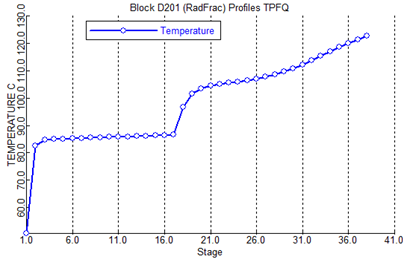
\includegraphics[scale=0.6]{example/tem.png}
	\caption{塔板温度分布图}
	\label{fig:tem}
\end{figure}

这里还有插入EPS图像和PDF图像的例子,如图\ref{fig:epspdf:a}和图\ref{fig:epspdf:b}。这里将EPS和PDF图片作为子图插入,每个子图有自己的小标题。子图标题使用subcaption宏包添加。

\begin{figure}[!htp]
  \centering
  \subcaptionbox{EPS 图像\label{fig:epspdf:a}}[3cm] %标题的长度,超过则会换行,如下一个小图。
    {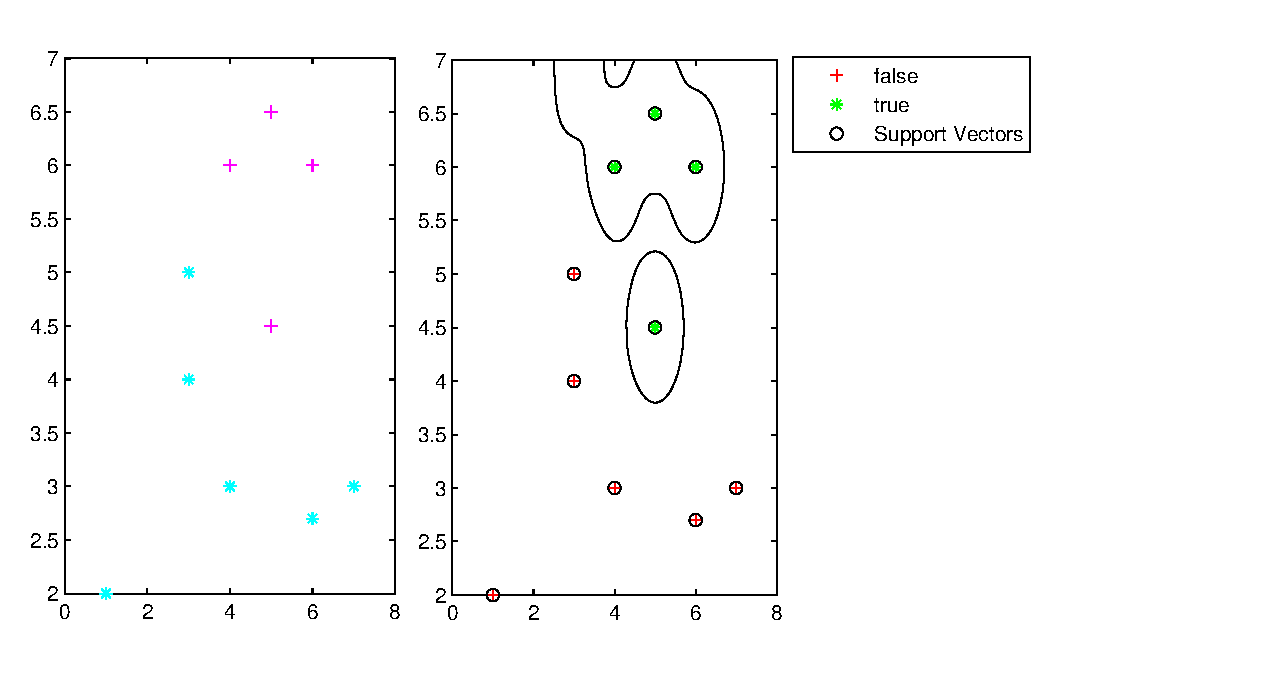
\includegraphics[height=4cm]{example/fig14.eps}}
  \hspace{4em}
  \subcaptionbox{PDF 图像。如果标题很长的话,它会自动换行\label{fig:epspdf:b}}
    {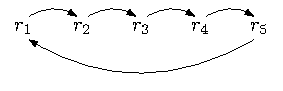
\includegraphics{example/permutation.pdf}}
  \caption{插入eps和pdf的例子(使用 subcaptionbox 方式)}
  \label{fig:pdfeps-subcaptionbox}
\end{figure}

\begin{figure}[!htp]
  \centering
  \begin{subfigure}{2.5cm}
    \centering
    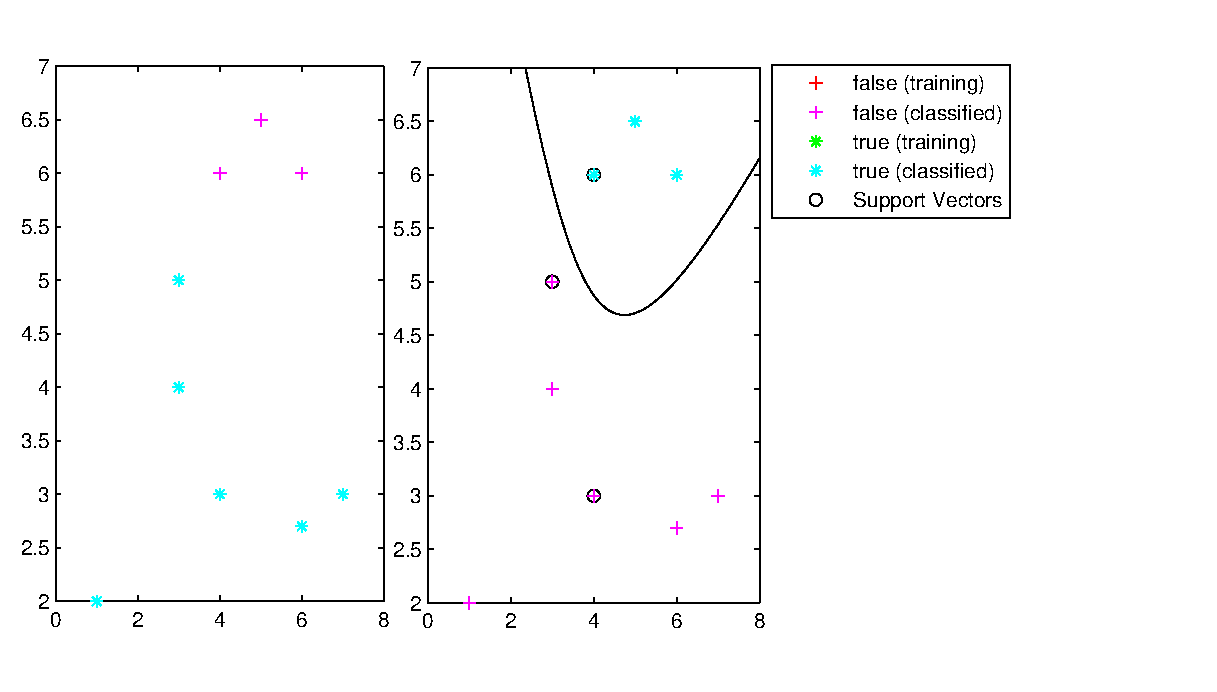
\includegraphics[height=3cm]{example/fig13.eps}
    \caption{EPS 图像}
  \end{subfigure}
  \hspace{4em}
  \begin{subfigure}{0.4\textwidth}
    \centering
    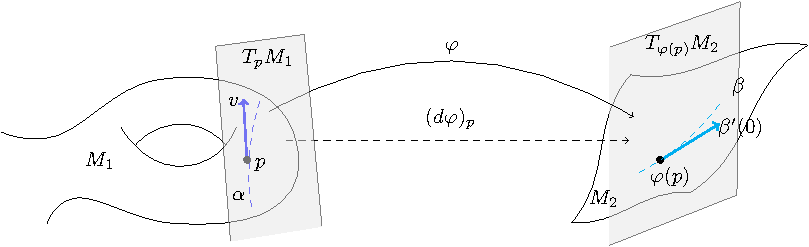
\includegraphics[height=2cm]{example/tangentmap.pdf}
    \caption{PDF 图像,注意这个图略矮些。subfigure中同一行的子图在顶端对齐。}
  \end{subfigure}
  \caption{插入eps和pdf的例子(使用 subfigure 方式)}
  \label{fig:pdfeps-subfigure}
\end{figure}

更多关于 \LaTeX 插图的例子可以参考\href{http://www.cs.duke.edu/junhu/Graphics3.pdf}{《\LaTeX 插图指南》}。

\subsection{绘制流程图}

图\ref{fig:flow_chart}是一张流程图示意。使用tikz环境,搭配四种预定义节点(\verb+startstop+、\verb+process+、\verb+decision+和\verb+io+),可以容易地绘制出流程图。
\begin{figure}[!htp]
    \centering
    \resizebox{6cm}{!}{\begin{tikzpicture}[node distance=2cm]
    \node (pic) [startstop] {待测图片};
    \node (bg) [io, below of=pic] {读取背景};
    \node (pair) [process, below of=bg] {匹配特征点对};
    \node (threshold) [decision, below of=pair, yshift=-0.5cm] {多于阈值};
    \node (clear) [decision, right of=threshold, xshift=3cm] {清晰?};
    \node (capture) [process, right of=pair, xshift=3cm, yshift=0.5cm] {重采};
    \node (matrix_p) [process, below of=threshold, yshift=-0.8cm] {透视变换矩阵};
    \node (matrix_a) [process, right of=matrix_p, xshift=3cm] {仿射变换矩阵};
    \node (reg) [process, below of=matrix_p] {图像修正};
    \node (return) [startstop, below of=reg] {配准结果};
     
    %连接具体形状
    \draw [arrow](pic) -- (bg);
    \draw [arrow](bg) -- (pair);
    \draw [arrow](pair) -- (threshold);

    \draw [arrow](threshold) -- node[anchor=south] {否} (clear);

    \draw [arrow](clear) -- node[anchor=west] {否} (capture);
    \draw [arrow](capture) |- (pic);
    \draw [arrow](clear) -- node[anchor=west] {是} (matrix_a);
    \draw [arrow](matrix_a) |- (reg);

    \draw [arrow](threshold) -- node[anchor=east] {是} (matrix_p);
    \draw [arrow](matrix_p) -- (reg);
    \draw [arrow](reg) -- (return);
\end{tikzpicture}
}
    \caption{绘制流程图效果}
    \label{fig:flow_chart}
\end{figure}

\section{表格}

这一节给出的是一些表格的例子,如表\ref{tab:firstone}所示。

\begin{table}[!hpb]
  \centering
  \caption{一个颇为标准的三线表格}
  \label{tab:firstone}
  \begin{tabular}{@{}llr@{}} \toprule
    \multicolumn{2}{c}{Item} \\ \cmidrule(r){1-2}
    Animal & Description & Price (\$)\\ \midrule
    Gnat & per gram & 13.65 \\
    & each & 0.01 \\
    Gnu & stuffed & 92.50 \\
    Emu & stuffed & 33.33 \\
    Armadillo & frozen & 8.99 \\ \bottomrule
  \end{tabular}
\end{table}

下面一个是一个更复杂的表格,用threeparttable实现带有脚注的表格,如表\ref{tab:footnote}。

\begin{table}[!htpb]
  \caption{一个带有脚注的表格的例子}
  \label{tab:footnote}
  \centering
  \begin{threeparttable}[b]
     \begin{tabular}{ccd{4}cccc}
      \toprule
      \multirow{2}{6mm}{total}&\multicolumn{2}{c}{20\tnote{1}} & \multicolumn{2}{c}{40} &  \multicolumn{2}{c}{60}\\
      \cmidrule(lr){2-3}\cmidrule(lr){4-5}\cmidrule(lr){6-7}
      &www & \multicolumn{1}{c}{k} & www & k & www & k \\ % 使用说明符 d 的列会自动进入数学模式,使用 \multicolumn 对文字表头做特殊处理
      \midrule
      &$\underset{(2.12)}{4.22}$ & 120.0140\tnote{2} & 333.15 & 0.0411 & 444.99 & 0.1387 \\
      &168.6123 & 10.86 & 255.37 & 0.0353 & 376.14 & 0.1058 \\
      &6.761    & 0.007 & 235.37 & 0.0267 & 348.66 & 0.1010 \\
      \bottomrule
    \end{tabular}
    \begin{tablenotes}
    \item [1] the first note.% or \item [a]
    \item [2] the second note.% or \item [b]
    \end{tablenotes}
  \end{threeparttable}
\end{table}

\section{参考文献管理}

 \LaTeX 具有将参考文献内容和表现形式分开管理的能力,涉及三个要素:参考文献数据库、参考文献引用格式、在正文中引用参考文献。
这样的流程需要多次编译:

\begin{enumerate}[noitemsep,topsep=0pt,parsep=0pt,partopsep=0pt]
	\item 用户将论文中需要引用的参考文献条目,录入纯文本数据库文件(bib文件)。
	\item 调用xelatex对论文模板做第一次编译,扫描文中引用的参考文献,生成参考文献入口文件(aux)文件。
	\item 调用bibtex,以参考文献格式和入口文件为输入,生成格式化以后的参考文献条目文件(bib)。
	\item 再次调用xelatex编译模板,将格式化以后的参考文献条目插入正文。
\end{enumerate}

参考文献数据库(thesis.bib)的条目,可以从Google Scholar搜索引擎\footnote{\url{https://scholar.google.com}}、CiteSeerX搜索引擎\footnote{\url{http://citeseerx.ist.psu.edu}}中查找,文献管理软件Papers\footnote{\url{http://papersapp.com}}、Mendeley\footnote{\url{http://www.mendeley.com}}、JabRef\footnote{\url{http://jabref.sourceforge.net}}也能够输出条目信息。

下面是在Google Scholar上搜索到的一条文献信息,格式是纯文本:

\begin{lstlisting}[caption={从Google Scholar找到的参考文献条目}, label=googlescholar, escapeinside="", numbers=none]
    @phdthesis{"白2008信用风险传染模型和信用衍生品的定价",
      title={"信用风险传染模型和信用衍生品的定价"},
      author={"白云芬"},
      year={2008},
      school={"上海交通大学"}
    } 
\end{lstlisting}

推荐修改后在bib文件中的内容为:

\begin{lstlisting}[caption={修改后的参考文献条目}, label=itemok, escapeinside="", numbers=none]
  @phdthesis{bai2008,
    title={"信用风险传染模型和信用衍生品的定价"},
    author={"白云芬"},
    date={2008},
    address={"上海"},
    school={"上海交通大学"}
  } 
\end{lstlisting}

按照教务处的要求,参考文献外观应符合国标GBT7714的要求\footnote{\url{http://www.cces.net.cn/guild/sites/tmxb/Files/19798_2.pdf}}。
在模板中,表现形式的控制逻辑通过biblatex-gb7714-2015包实现\footnote{\url{https://www.ctan.org/pkg/biblatex-gb7714-2015}},基于{Bib\LaTeX}管理文献。在目前的多数TeX发行版中,可能都没有默认包含biblatex-gb7714-2015,需要手动安装。

正文中引用参考文献时,用\verb+\cite{key1,key2,key3...}+可以产生“上标引用的参考文献”,
如\cite{Meta_CN,chen2007act,DPMG}。
使用\verb+\parencite{key1,key2,key3...}+则可以产生水平引用的参考文献,例如\parencite{JohnD,zhubajie,IEEE-1363}。
请看下面的例子,将会穿插使用水平的和上标的参考文献:关于书的\parencite{Meta_CN,JohnD,IEEE-1363},关于期刊的\cite{chen2007act,chen2007ewi},
会议论文\parencite{DPMG,kocher99,cnproceed},
硕士学位论文\parencite{zhubajie,metamori2004},博士学位论文\cite{shaheshang,FistSystem01,bai2008},标准文件\parencite{IEEE-1363},技术报告\cite{NPB2},电子文献\parencite{xiaoyu2001, CHRISTINE1998},用户手册\parencite{RManual}。

总结一些注意事项:
\begin{itemize}
\item 参考文献只有在正文中被引用了,才会在最后的参考文献列表中出现;
\item 参考文献“数据库文件”bib是纯文本文件,请使用UTF-8编码,不要使用GBK编码;
\item 参考文献条目中默认通过date域输入时间。兼容使用year域时会产生编译warning,可忽略。
\end{itemize}

\section{用listings插入源代码}

\begin{lstlisting}[language={C}, caption={一段C源代码}]
#include <stdio.h>
#include <unistd.h>
#include <sys/types.h>
#include <sys/wait.h>

int main() {
  pid_t pid;

  switch ((pid = fork())) {
  case -1:
    printf("fork failed\n");
    break;
  case 0:
    /* child calls exec */
    execl("/bin/ls", "ls", "-l", (char*)0);
    printf("execl failed\n");
    break;
  default:
    /* parent uses wait to suspend execution until child finishes */
    wait((int*)0);
    printf("is completed\n");
    break;
  }

  return 0;
}
\end{lstlisting}

\section{用algorithm和algorithmicx宏包插入算法描述}

algorithmicx 比 algorithmic 增加了一些命令。
示例如算法\ref{algo:sum_100}和算法\ref{algo:merge_sort},
后者的代码来自\href{http://hustsxh.is-programmer.com/posts/38801.html}{xhSong的博客}。
algorithmicx的详细使用方法见\href{http://mirror.hust.edu.cn/CTAN/macros/latex/contrib/algorithmicx/algorithmicx.pdf}{官方README}。
使用算法宏包时,算法出现的位置很多时候不按照tex文件里的书写顺序, 
需要强制定位时可以使用\verb+\begin{algorithm}[H]+
\footnote{http://tex.stackexchange.com/questions/165021/fixing-the-location-of-the-appearance-in-algorithmicx-environment}
\begin{algorithm}
% \begin{algorithm}[H] % 强制定位
\caption{求100以内的整数和}
\label{algo:sum_100}
\begin{algorithmic}[1] %每行显示行号
\Ensure 100以内的整数和 % 输出
\State $sum \gets 0$
\For{$i = 0 \to 100$}
    \State $sum \gets sum + i$
  \EndFor
\end{algorithmic}
\end{algorithm}
         % for testing
%% for testing list of symbols
%% To add the symbols to the list of symbols, need to use $\gls{t}$ in the contents
%% which will create hyperlink to the section of listofsymbols
%% To add the description of the symbols, one must add the entry in "symbols.tex" file
\chapter{Sample}
Reference symbols: $\gls{x}$, $\gls{v}$, $\gls{a}$, $\gls{t}$,
$\gls{F}$,$\gls{xx}$.

%%%%%%%%%%%%%%%%%%%%%%%%%%%%%%%%%%%%%%%%%%%%%%%%%%%%%%%%%%%%%%%%%%%%%%%%%%%%%%% 
% bibliography                                                                %
%%%%%%%%%%%%%%%%%%%%%%%%%%%%%%%%%%%%%%%%%%%%%%%%%%%%%%%%%%%%%%%%%%%%%%%%%%%%%%% 
\bibliographystyle{tsien} % bibliography style, for example: plain, style "tsien" is user cumstomized
\bibliography{biblio}       % bib file name 

\end{document}
%%% the following three lines of comments are used for emacs auctex users, each 
%%% input file contains them. One can compile tex file on any buffer of them

%%% Local Variables:
%%% mode: latex
%%% TeX-master: t
%%% End:
